\documentclass[a4paper,twocolumn,gsifonts,twoside]{gsipaper}
\usepackage{a4wide,gsiindex,helvet}
\usepackage[english]{babel}
\usepackage{amsmath,amsfonts,amssymb,verbatim,float}
\usepackage[pdftex]{graphicx}
\usepackage{textcomp}
\usepackage{subfigure}
\usepackage{ulem}
\usepackage{soul} 
\usepackage{footnote}
\usepackage{cool}
\usepackage{eulervm}

\let\oldmb\mathbold
\protected\def\mathbold{\oldmb}

\begin{document}
\title{Heavy-flavour production in proton-proton collisions at $\mathbold{\sqrt{s} = 7}$ TeV}
\subtitle{\centering{Estimation of $\mathbold{\gamma}$, \space $\mathbold{\pi^{0}}$ and $\mathbold{\eta}$ ratios in the photonic background}}

\abstract{The heavy-flavour production in proton-proton collisions is an important testing ground for perturbative QCD, the field theory for the 
strong interaction. \\One way of measuring heavy-flavour hadrons is via the leptons originating from their decays. The aim of this study 
is to evaluate the ratios between the photon conversions, and the $\pi^{0}$ and $\eta$ Dalitz decays, which are the main sources of 
the background, in proton-proton collisions at $\sqrt{s} = 7$ TeV. \\
In first analysis the amount of these sources has been derived from a simulation, using the MC truth. \\Then the MC information has been 
ignored, in order to approach a realistic analysis strategy to be performed with real data. For this purpose the combinatorial method 
has been used; it consists in calculating the invariant mass of an ”inclusive” $e^{\pm}$ , for which stringent cuts are required to be 
sure that its track belongs to an $e^{\pm}$, combined with an ”associated” one, for which only relaxed cuts are required to maximise the 
efficiency. Then the photonic signal has been obtained subtracting the like-sign ($e^{\pm}e^{\pm}$) distribution, which only contains 
the combinatorial information, from the unlike-sign ($e^{\pm}e^{\mp}$) distribution, which has both the photonic signal and the 
combinatorial background; finally the quantitative contributions of the main sources are derived from a fit  of the resulting photonic 
signal.}

\author{Fabrizio Grosa}        
\address{Universit\`{a} degli studi di Torino, fabrizio.grosa@studenti.unito.it}

\maketitle

\section{Introduction}
\subsection{Quark-gluon plasma}

\begin{figure}[htb]
\begin{center}
\advance\leftskip-1cm
\advance\rightskip-0.cm
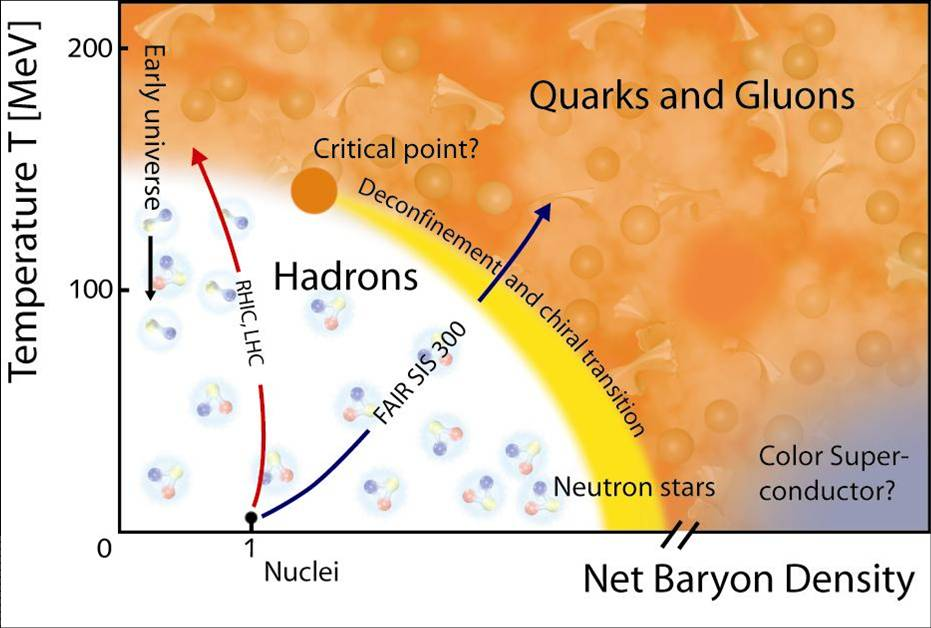
\includegraphics[scale = 0.4]{QCD_phase_diagram.jpg}
\caption{Phase diagram of hadronic matter and the hadron gas - quark-gluon plasma phase transition.}
\label{diagram}
\end{center}
\end{figure}

Quantum chromodynamics (QCD) predicts that under extreme conditions of very high temperature
or baryo-chemical potential $\mu_{B}$ hadronic matter transits to a deconfined phase of matter called \textit{``quark-gluon plasma``}
(QGP), in which quarks and gluons are not bound in hadrons.\\

The QGP is thought to have permeated the universe for few $\mu s$ after the Big Bang. Experimentally, it can be created in 
ultra-relativistic heavy-ion collisions.\\
These collisions create a so called \textit{fireball} of interacting quarks and gluons above the critical temperature, 
which first reaches the thermal equilibrium, and then quickly expands and cools down. During the cooling starts the 
\textit{hadronization}, or rather quarks and gluons become again confined and form hadrons.\\
The last phases are the \textit{chemical freeze-out} and the \textit{kinetic freeze-out}, where, 
respectively, inelastic and elastic processes cease.

\subsection{Heavy-flavour production}
The production of hadrons which contain heavy quarks (charm or beauty) is an important probe for the QGP. It happens exclusively 
through initial hard partonic scattering processes when the medium is more dense, because of their higher mass. Heavy quarks lose 
energy differently than the light quarks in the QGP and therefore they are a signature of the deconfinement, 
and their behaviour in the medium is useful to characterise the medium itself.\\

Hadrons carrying heavy flavour can decay by weak interaction, through a \textit{''semileptonic decay``}, in which one lepton (and the 
corresponding neutrino) is produced in addition to one or more hadrons.\\
Therefore the electrons/positrons are measured \textit{inclusively}, coming from both the heavy-flavour hadrons decays and the 
background sources. In Fig. \ref{cocktail} \space is shown the $p_{T}$ spectrum for the $e^{\pm}$ measured. 
After subtracting the background $e^{\pm}$ the remaining $p_{T}$ spectrum contains only the electrons from heavy-flavour decays.
It is then important to estimate the background for these decays to quantify the heavy-flavour production. \\

\begin{figure}[tb]
\begin{center}
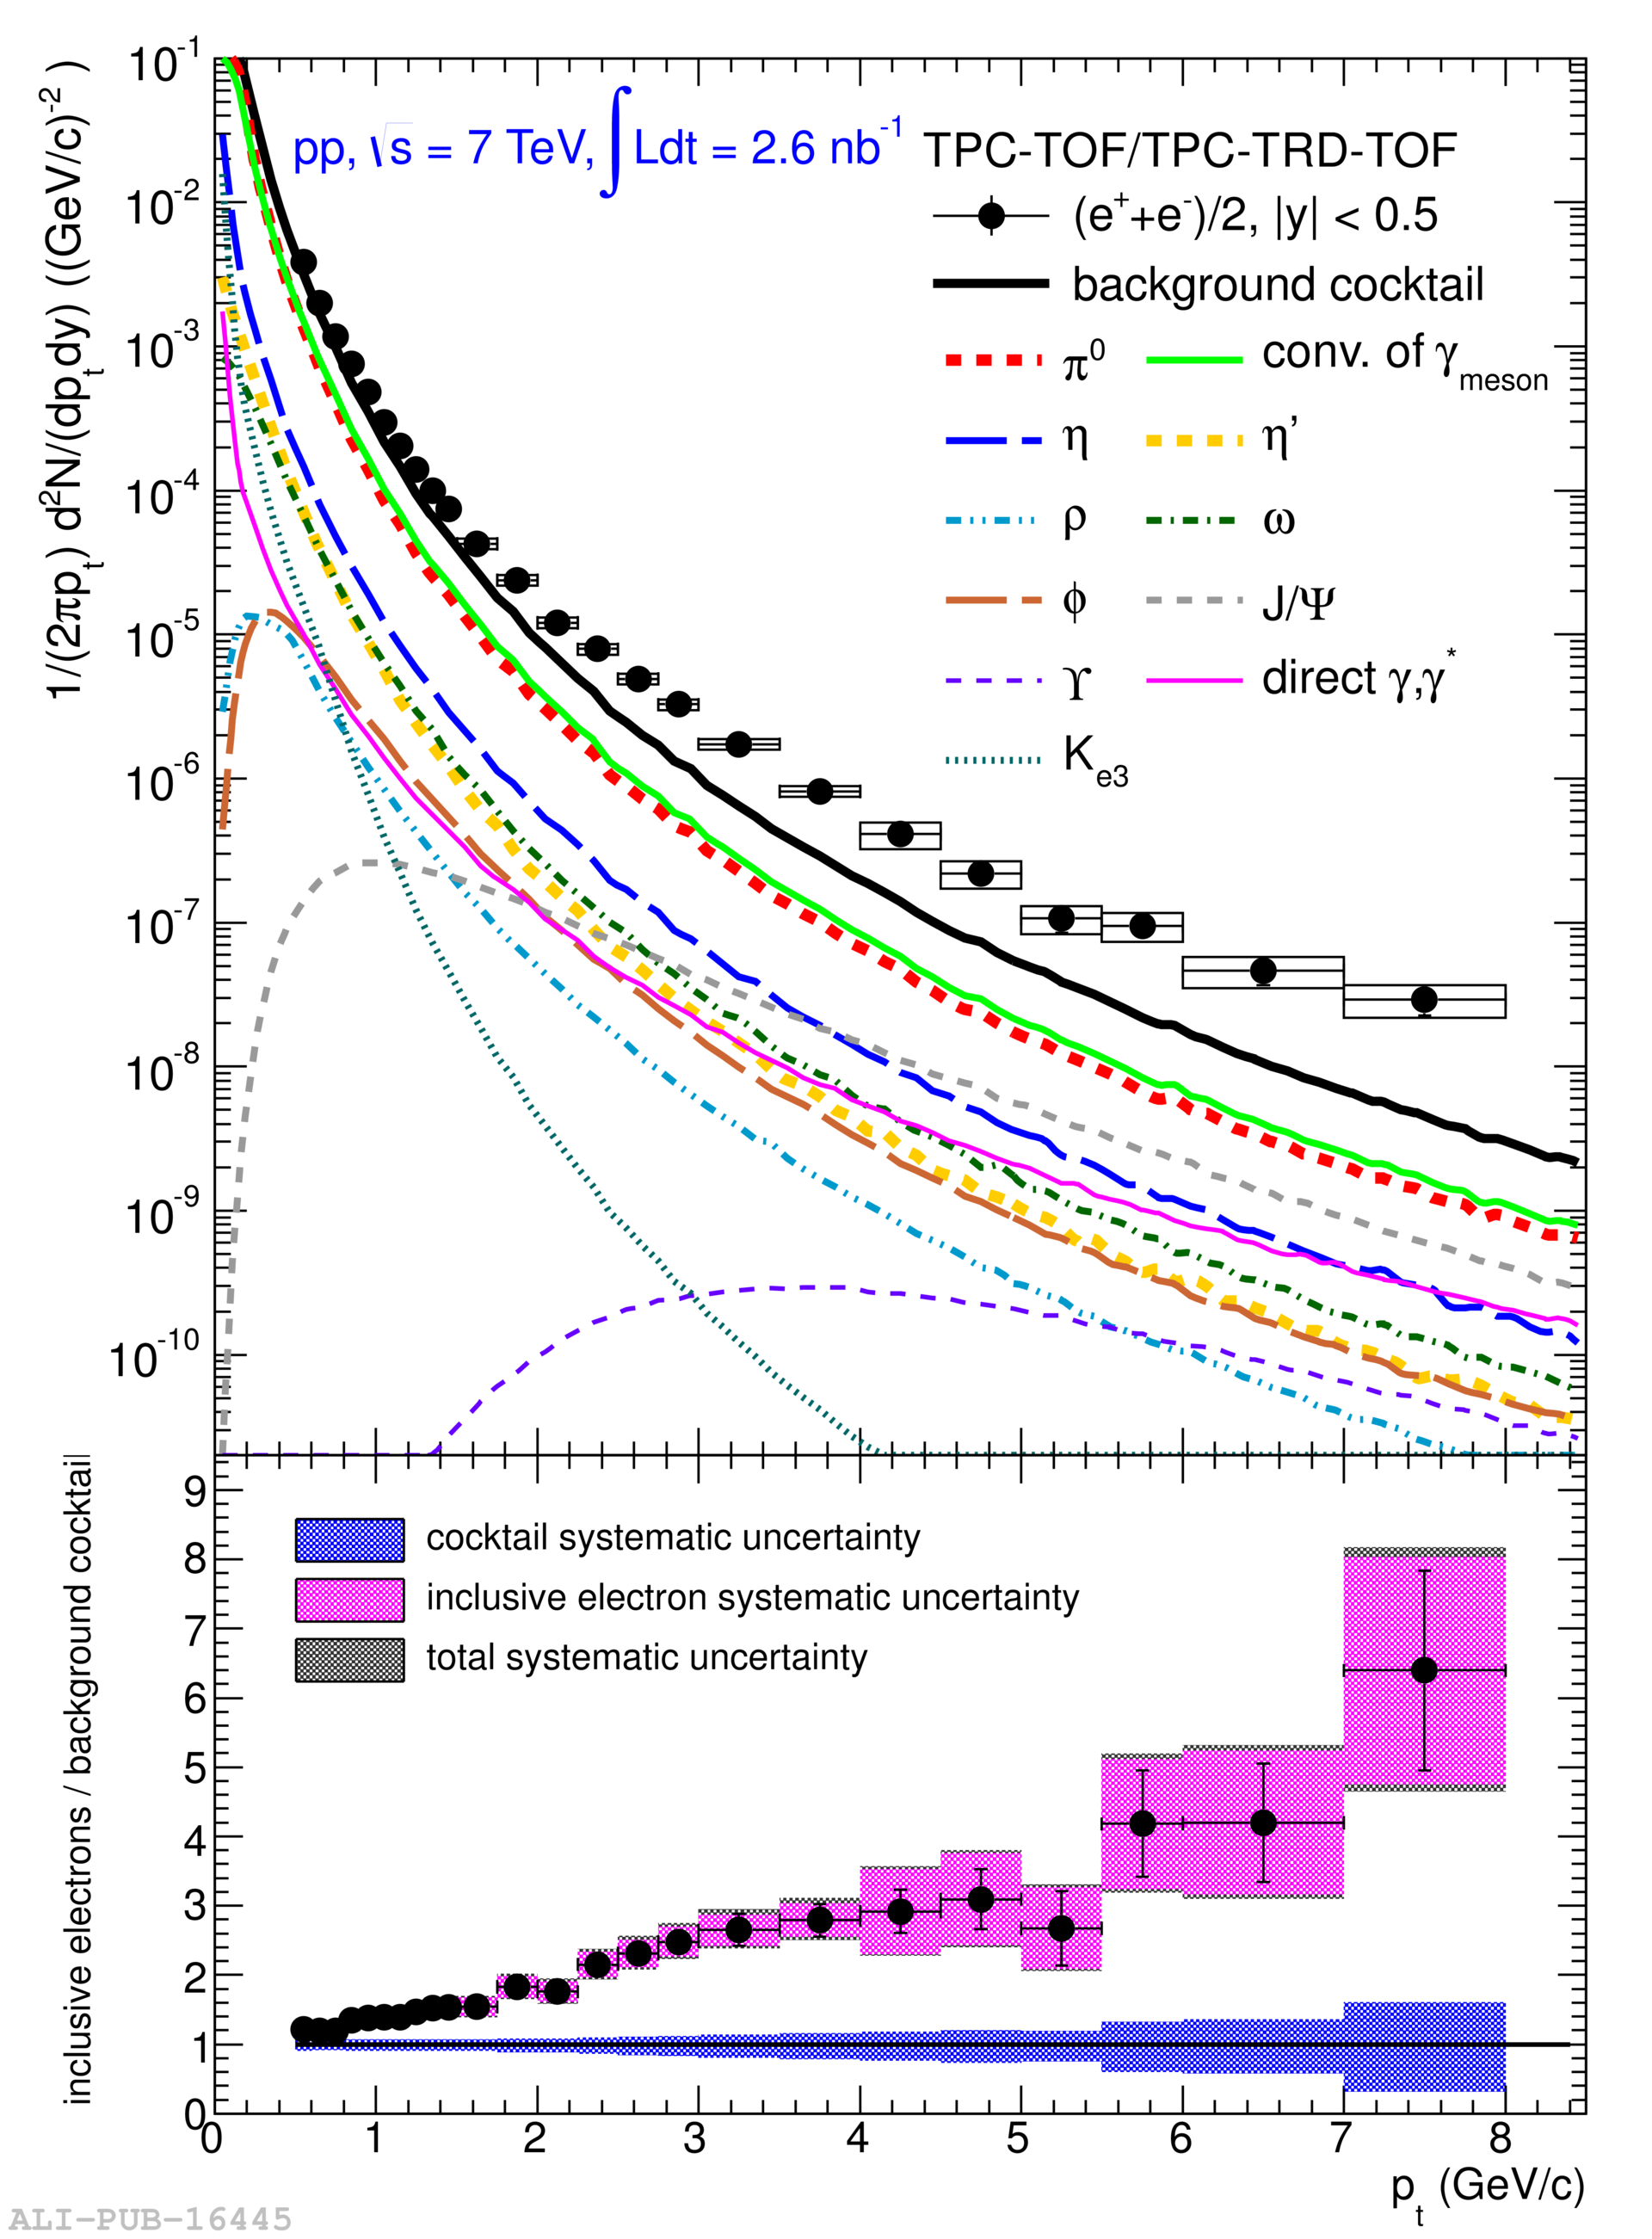
\includegraphics[scale = 0.12]{2013-Jan-03-inclusive_versus_cocktail_combined_mult.png}
\caption{The inclusive $e^{\pm}$ measurement with the sources of the background calculated with the cocktail method 
\cite{Averbeck:2013oga} for proton-proton collisions at $\sqrt{s} = 7$ TeV.}
\label{cocktail}
\end{center}
\end{figure}

\subsection{The photonic background}
\label{section:photonic}
For the low $p_{T}$ region the dominant contributions of the background are of so called \textit{photonic} origin. \\
The main sources for this photonic background are the photon conversions ($\gamma\rightarrow e^{+}e^{-}$) and the $\pi^{0}$ and $\eta$
Dalitz decays ($\pi^{0} \rightarrow e^{+}e^{-}\gamma$ and $\eta \rightarrow e^{+}e^{-}\gamma$), which are the major contribution
for the low $p_{T}$ region (80\%\textdiv \space 95\%). \\

The aim of the following study is to quantify the relative amount of those three sources, especially the ratio between photons and 
$\pi_{0}$ and $\eta$ mesons, for proton-proton collisions at $\sqrt{s} = 7$ TeV. Proton-proton collisions are important to be 
investigated, despite in these the QGP cannot be created, because they represent the reference system for Pb-Pb collisions.

\subsection{The ALICE detector}
The LHC is the largest hadron collider in the world, and it is located at CERN, on the Swiss-France border, close to Geneva.\\
The four large experiments at LHC are:
\begin{itemize}
 \item \textbf{ALICE} (\textbf{A} \textbf{L}arge \textbf{I}on \textbf{C}ollider \textbf{E}xperiment)
 \item \textbf{CMS} (The \textbf{C}ompact \textbf{M}uon \textbf{S}olenoid)
 \item \textbf{ATLAS} (\textbf{A} \textbf{T}oroidal \textbf{L}HC \textbf{A}pparatu\textbf{S})
 \item \textbf{LHCb} (\textbf{LHC} \textbf{b}eauty experiment)
\end{itemize}

The ALICE detector, which is shown in Fig. \ref{ALICE}, is dedicated to heavy-ion collisions and therefore to the study of the QGP.
It is 26 m long, 16 m wide and weights more than 10000 tn. The magnet surrounding the central barrel creates an homogeneus magnetic 
field of B = 0.5 T, which allows the measurement of the momentum of the charged particles.\\

\begin{figure*}[tb]
\begin{center}
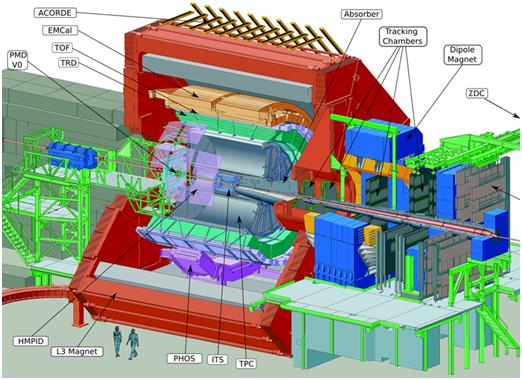
\includegraphics[scale = 1.1]{ALICE_detector.jpg}
\caption{The ALICE schematic geometry}
\label{ALICE}
\end{center}
\end{figure*}

ALICE is composed by several subdetectors. The four cylindrical tracking detectors in the central barrel (Fig.\ref{ALICE_section}) are 
the \textbf{I}nner \textbf{T}racking \textbf{S}ystem (ITS), the \textbf{T}ime \textbf{P}rojection \textbf{C}hamber (TPC), the 
\textbf{T}ime-\textbf{O}f-\textbf{F}light detector (TOF) and the \textbf{T}ransition \textbf{R}adiation \textbf{D}etector (TDR). 
In the central barrel there are also two electromagnetic calorimeters, the \textbf{E}lectro\textbf{M}agnetic \textbf{Cal}orimeter (EMCal)
and the \textbf{PHO}ton \textbf{S}pectrometer (PHOS). Equally in the central part, but more externally, there are the \textbf{P}hoton 
\textbf{M}ultiplicity \textbf{D}etector (PMD) and the \textbf{H}igh \textbf{M}omentum \textbf{P}article \textbf{I}dentification 
\textbf{D}etector (HMPID). In forward rapidity there are the T0 detector, which generates the start time for the TOF, and the V0 
detector, which provides a minimum bias trigger for the central barrel detectors.
Finally in the right side of Fig. \ref{ALICE} we can see the muon spectrometer, which is used to study the heavy quarkonia,
and the \textbf{Z}ero \textbf{D}egree \textbf{C}alorimeter (ZDC) which consists in two pairs of hadron calorimeters, for neutrons (ZN), 
and protons (ZP).

For this analysis only the ITS and the TPC will be used for the selection of the tracks.

\begin{figure}[htb]
\begin{center}
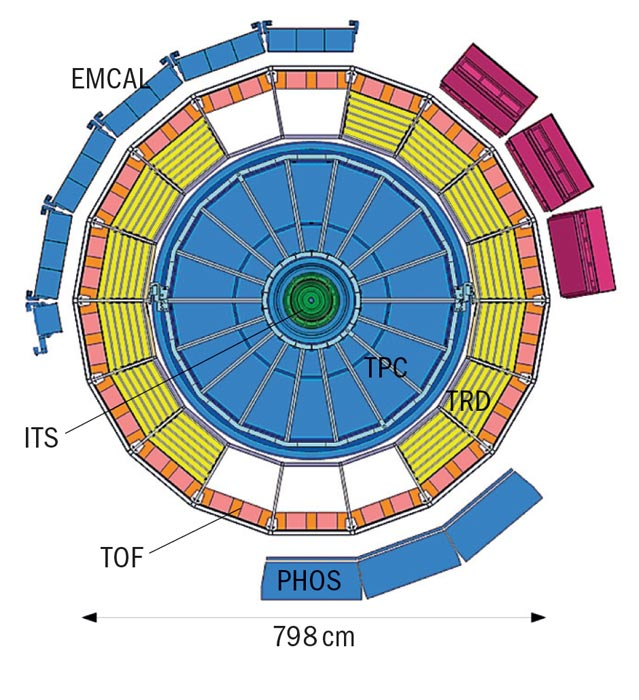
\includegraphics[scale = 0.25]{ITS_TPC.jpg}
\caption{The ALICE schematic central barrel detectors in cross section}
\label{ALICE_section}
\end{center}
\end{figure}

\newpage
\subsubsection{Inner Tracking System}
The ITS is the first subdetector reached by the particles originating in the collisions. The ITS consists of six layers of three 
different silicon detector types: the \textbf{S}ilicon \textbf{P}ixel \textbf{D}etector (SPD), the \textbf{S}ilicon \textbf{D}rift
\textbf{D}etector (SDD) and the \textbf{S}ilicon Micro\textbf{S}trip \textbf{D}etector (SSD). The main purpose of this detector is to 
separate tracks coming from the primary vertex, from those which are coming from the secondary verteces.

\subsubsection{Time Projection Chamber}
The TPC is the main tracking detector of ALICE. It has a diameter of about 5.6 m and length of 5.1 m. The drift region is filled with 
a gas mixture of $Ne$, $CO_{2}$ and $N_{2}$. Together with the ITS, the Time Projection Chamber provides the charged particle track 
reconstruction, the primary and secondary vertices reconstruction and the particle identification, via the measurement of the energy 
loss $dE/dx$.

\section{Data analysis}
\subsection{Data sample}
For this analysis MC data for proton-proton collisions at $\sqrt{s} = 7$ TeV (LHC10f6a) have been used: they are generated with PYTHIA 6
and their behaviour in the detectors (ITS, TPC and TOF) has been simulated with GEANT 3\footnote{\textbf{GE}ometry \textbf{AN}d 
\textbf{T}racking package}.\\

\begin{figure}[h]
\begin{center}
\advance\leftskip-0.5cm
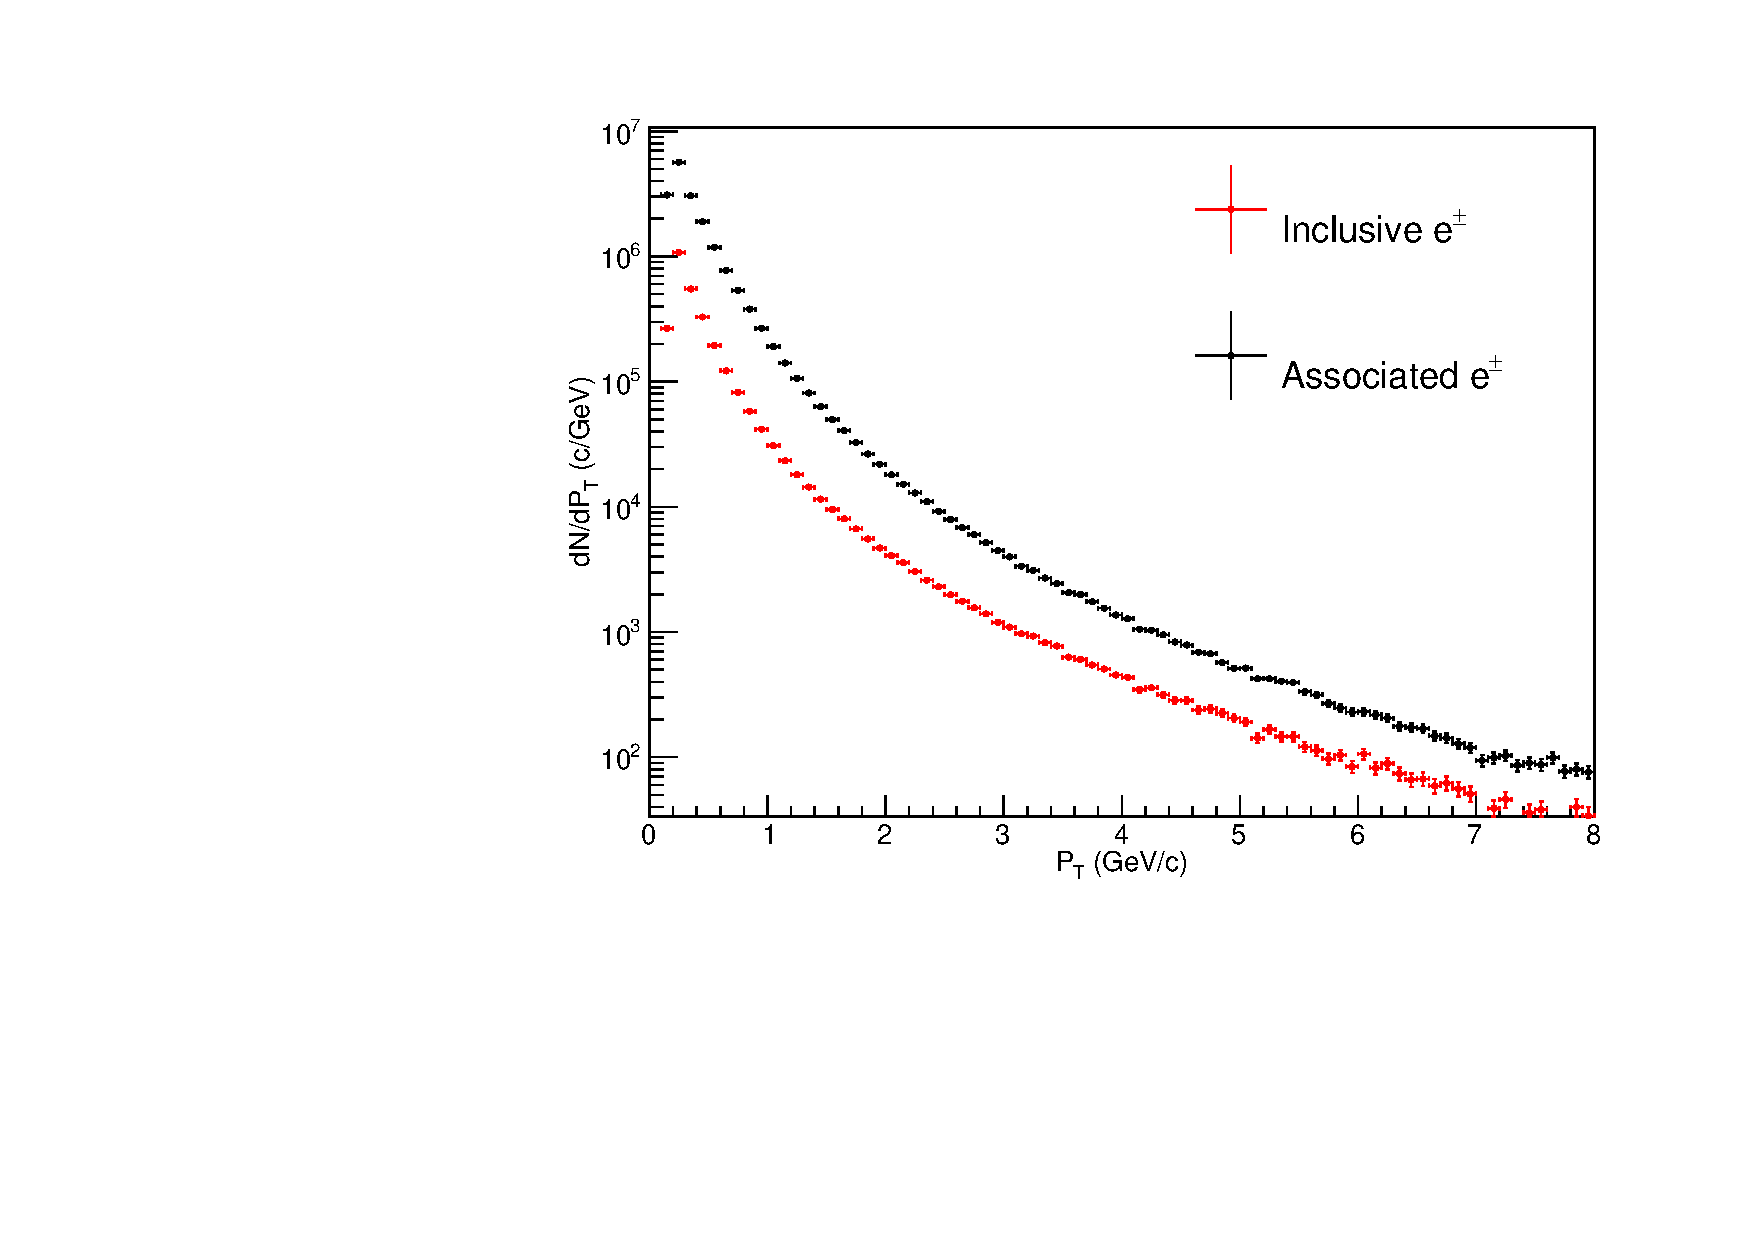
\includegraphics[scale = 0.42]{incl-ass.pdf}
\caption{The inclusvie and associated $e^{\pm}$ $p_{T}$ spectrum}
\label{pt_spectrum}
\end{center}
\end{figure}

\subsection{Tracks selection}
The idea of this analysis method is to combine an "inclusive" $e^{\pm}$, whose track is surely related to an electron, 
with an "associated" $e^{\pm}$, for which less stringent cuts are required to maximise the efficiency.\\
The cuts applied to the reconstructed tracks, for "inclusive" and "associated" $e^{\pm}$, are shown in the following table:

\begin{table}[htpb]
\center
\caption{Cuts applied for "inclusive" and "associated" $e^{\pm}$}\label{cuts}
\fontsize{10}{3}
\scalebox{0.8}{
\begin{tabular}{|c|c|c|}
  \hline
  \raisebox{0pt}[10pt][4pt]{} &
  \raisebox{0pt}[12pt][4pt]{\textbf{inc e$^{\pm}$}} &
  \raisebox{0pt}[12pt][4pt]{\textbf{ass e$^{\pm}$}} \\
  \hline
  \raisebox{0pt}[10pt][4pt]{$\chi^{2}/$cluster} &
  \raisebox{-8pt}[10pt][4pt]{$<$ 4} &
  \raisebox{-8pt}[10pt][4pt]{$<$ 4} \\
  \raisebox{0pt}[10pt][4pt]{in the TPC track fit} &
  \raisebox{0pt}[10pt][4pt]{} &
  \raisebox{0pt}[10pt][4pt]{} \\
  \hline
  \raisebox{0pt}[10pt][4pt]{ITS/TPC refit} &
  \raisebox{0pt}[10pt][4pt]{yes} &
  \raisebox{0pt}[10pt][4pt]{yes} \\
  \hline
  \raisebox{0pt}[10pt][4pt]{number of TPC clusters} &
  \raisebox{0pt}[10pt][4pt]{$\geq$ 120} &
  \raisebox{0pt}[10pt][4pt]{$\geq$ 100} \\
  \hline
  \raisebox{0pt}[10pt][4pt]{number of ITS clusters} &
  \raisebox{0pt}[10pt][4pt]{$\geq$ 4} &
  \raisebox{0pt}[10pt][4pt]{$\geq$ 2} \\
  \hline
  \raisebox{0pt}[10pt][4pt]{number of TPC cluster} &
  \raisebox{-8pt}[10pt][4pt]{$\geq$ 80} &
  \raisebox{-8pt}[10pt][4pt]{$\geq$ 80} \\
  \raisebox{0pt}[10pt][4pt]{for PID} &
  \raisebox{0pt}[10pt][4pt]{} &
  \raisebox{0pt}[10pt][4pt]{} \\
  \hline
  \raisebox{0pt}[10pt][4pt]{TPC Ratio found/findable} &
  \raisebox{-8pt}[10pt][4pt]{$>$ 0.6} &
  \raisebox{-8pt}[10pt][4pt]{-} \\
  \raisebox{0pt}[10pt][4pt]{clusters} &
  \raisebox{0pt}[10pt][4pt]{} &
  \raisebox{0pt}[10pt][4pt]{} \\
  \hline
  \raisebox{0pt}[10pt][4pt]{Transverse momentum} &
  \raisebox{0pt}[10pt][4pt]{0.1 $<p_{T}<$ 20} &
  \raisebox{0pt}[10pt][4pt]{-} \\
  \hline
  \raisebox{0pt}[10pt][4pt]{Pseudorapidity} &
  \raisebox{0pt}[10pt][4pt]{$\mid\eta\mid<$ 0.8} &
  \raisebox{0pt}[10pt][4pt]{$\mid\eta\mid<$ 0.8} \\
  \hline
  \raisebox{0pt}[10pt][4pt]{Reject Kink daughter} &
  \raisebox{0pt}[10pt][4pt]{yes} &
  \raisebox{0pt}[10pt][4pt]{yes} \\
  \hline
  \raisebox{0pt}[10pt][4pt]{DCA in $\mid\vec{r}\mid$-direction [cm]} &
  \raisebox{0pt}[10pt][4pt]{$<$ 1} &
  \raisebox{0pt}[10pt][4pt]{$<$ 1} \\
  \hline
  \raisebox{0pt}[10pt][4pt]{DCA in z-direction [cm]} &
  \raisebox{0pt}[10pt][4pt]{$<$ 2} &
  \raisebox{0pt}[10pt][4pt]{$<$ 2} \\
  \hline
  \raisebox{0pt}[10pt][4pt]{ITS SPD layer hit} &
  \raisebox{0pt}[10pt][4pt]{First} &
  \raisebox{0pt}[10pt][4pt]{-} \\
  \hline
  \end{tabular}}
\end{table}
Finally, using the MC truth information, only the tracks that really belong to $e^{\pm}$ are selected for both "inclusive" 
and "associated" $e^{\pm}$.
In Fig. \ref{pt_spectrum} is shown the row $p_{T}$ spectrum for both electrons/positrons samples. As we can see the associated $e^{\pm}$
are one order of magnitude more than the inclusive ones, therefore more statistics for the analysis is available.

\subsection{Invariant mass analysis}

Using the conservation of the four-momentum $p = (E, \vec{p})$, and the following equation derived from the Special Relativity:
\begin{equation}
 m^{2} = E^{2}-\vec{p}^{2} \equiv p^{2}  
 \label{mass}
\end{equation}

it is possible to reconstruct the mass of a particle from its decay products \\(in our case they will be $e^{\pm}e^{\mp}$, 
or equivalently $e^{\pm}e^{\pm}$), using the following relation:

\begin{align} 
\setlength{\jot}{12pt} 
m_{ee} &= \sqrt{(p_{1}+p_{2})^{2}} \\ \nonumber
&= \sqrt{(E_{1}+E_{2})^{2}-(\vec{p_{1}}+\vec{p_{2}})^{2}}. 
\label{mee}
\end{align}

\begin{figure*}[tb]
\begin{center}
\advance\leftskip-0.5cm
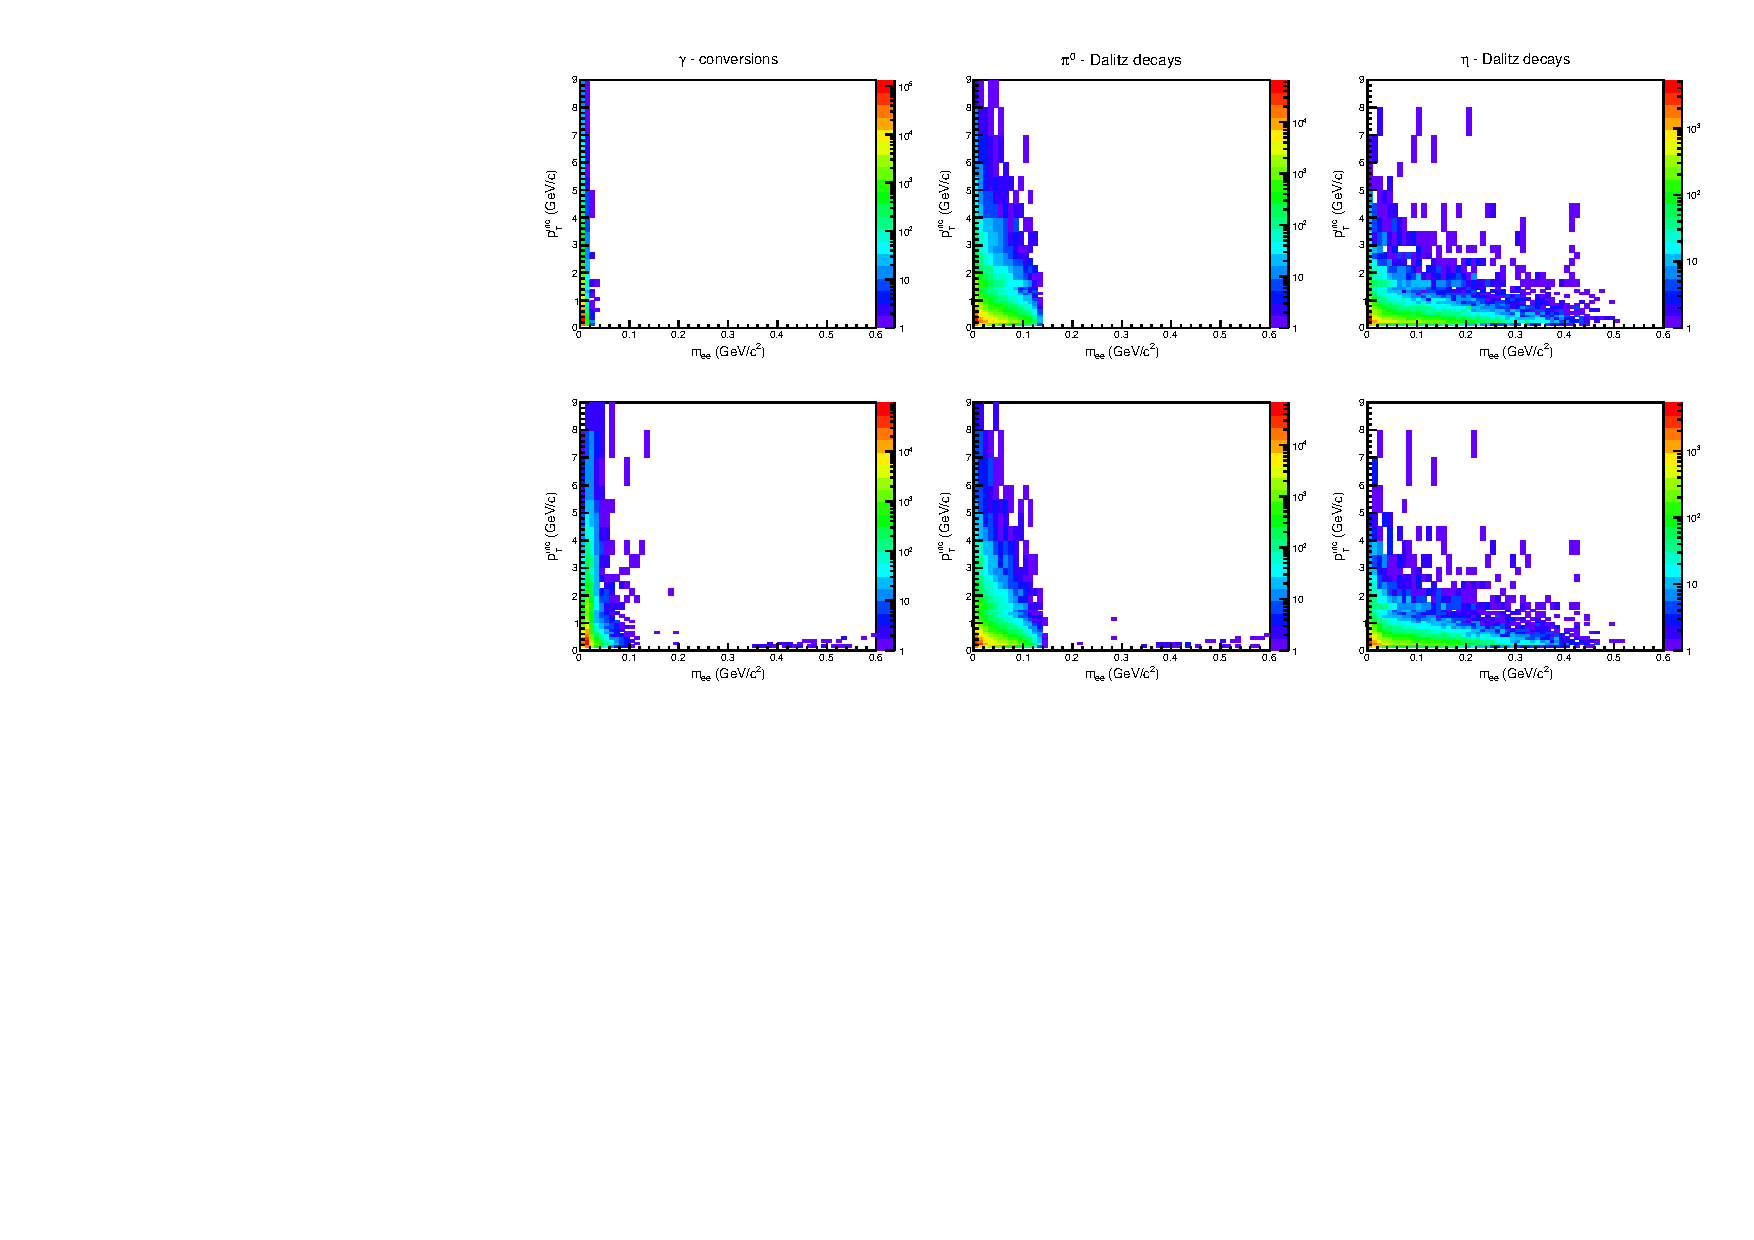
\includegraphics[scale = 0.8]{ptmee2.pdf}
\caption{The correlation between the transverse momentum of the inclusive electron ($p_{T}^{inc}$) and the invariant mass of the 
$e^{+}e^{-}$ pair coming from the MC information, with MC truth parameters (upper plots) and ESD reconstructed parameters (lower plots).}
\label{corr}
\end{center}
\end{figure*}

The indices 1 and 2 stand for the two candidates and the energy is calculated from the mass of the daughter particles (in this case
\\$m_{e} =$ 0.511 MeV), using the equation (\ref{mass}) inverted:

\begin{equation}
 E_{i} = \sqrt{m_{e}^{2}+\vec{p}_{i}^{2}}
 \label{energy}
\end{equation}

\vspace{0.3cm}
because $E_{i}$ is not directly measured.

\section{Photonic background with MC information}
Using the MC information it is possible to select every $e^{+}e^{-}$ pair which comes from one of the main sources listed before
(photon conversions or $\pi^{0}$ and $\eta$ Dalitz decays), and then to obtain their kinematic parameters.\\ 

Every measured particle is described by several parameters which determine its kinematic and track.\\
The initial observables, which describe the particle how it was originally created, are known from the MC truth.
From ESD\footnote{\textbf{E}vent \textbf{S}ummary \textbf{D}ata} it is possible to obtain the parameters after the interaction
of the particle with the material of the detectors,  and its track has been reconstructed from the measured information. 

In Fig. \ref{corr} is shown the correlation between the transverse momentum of the inclusive electron and the 
invariant mass of the $e^{+}e^{-}$ pair. As we can notice the majority of the counts are in the low $p_{T}$ and $m_{ee}$ region, in fact 
the photonic sources are domimant for low transverse momentum, as described in section \ref{section:photonic}.

\subsection{Invariant mass distributions from MC truth}
\begin{figure*}[tb]
\begin{center}
\advance\leftskip-0.5cm
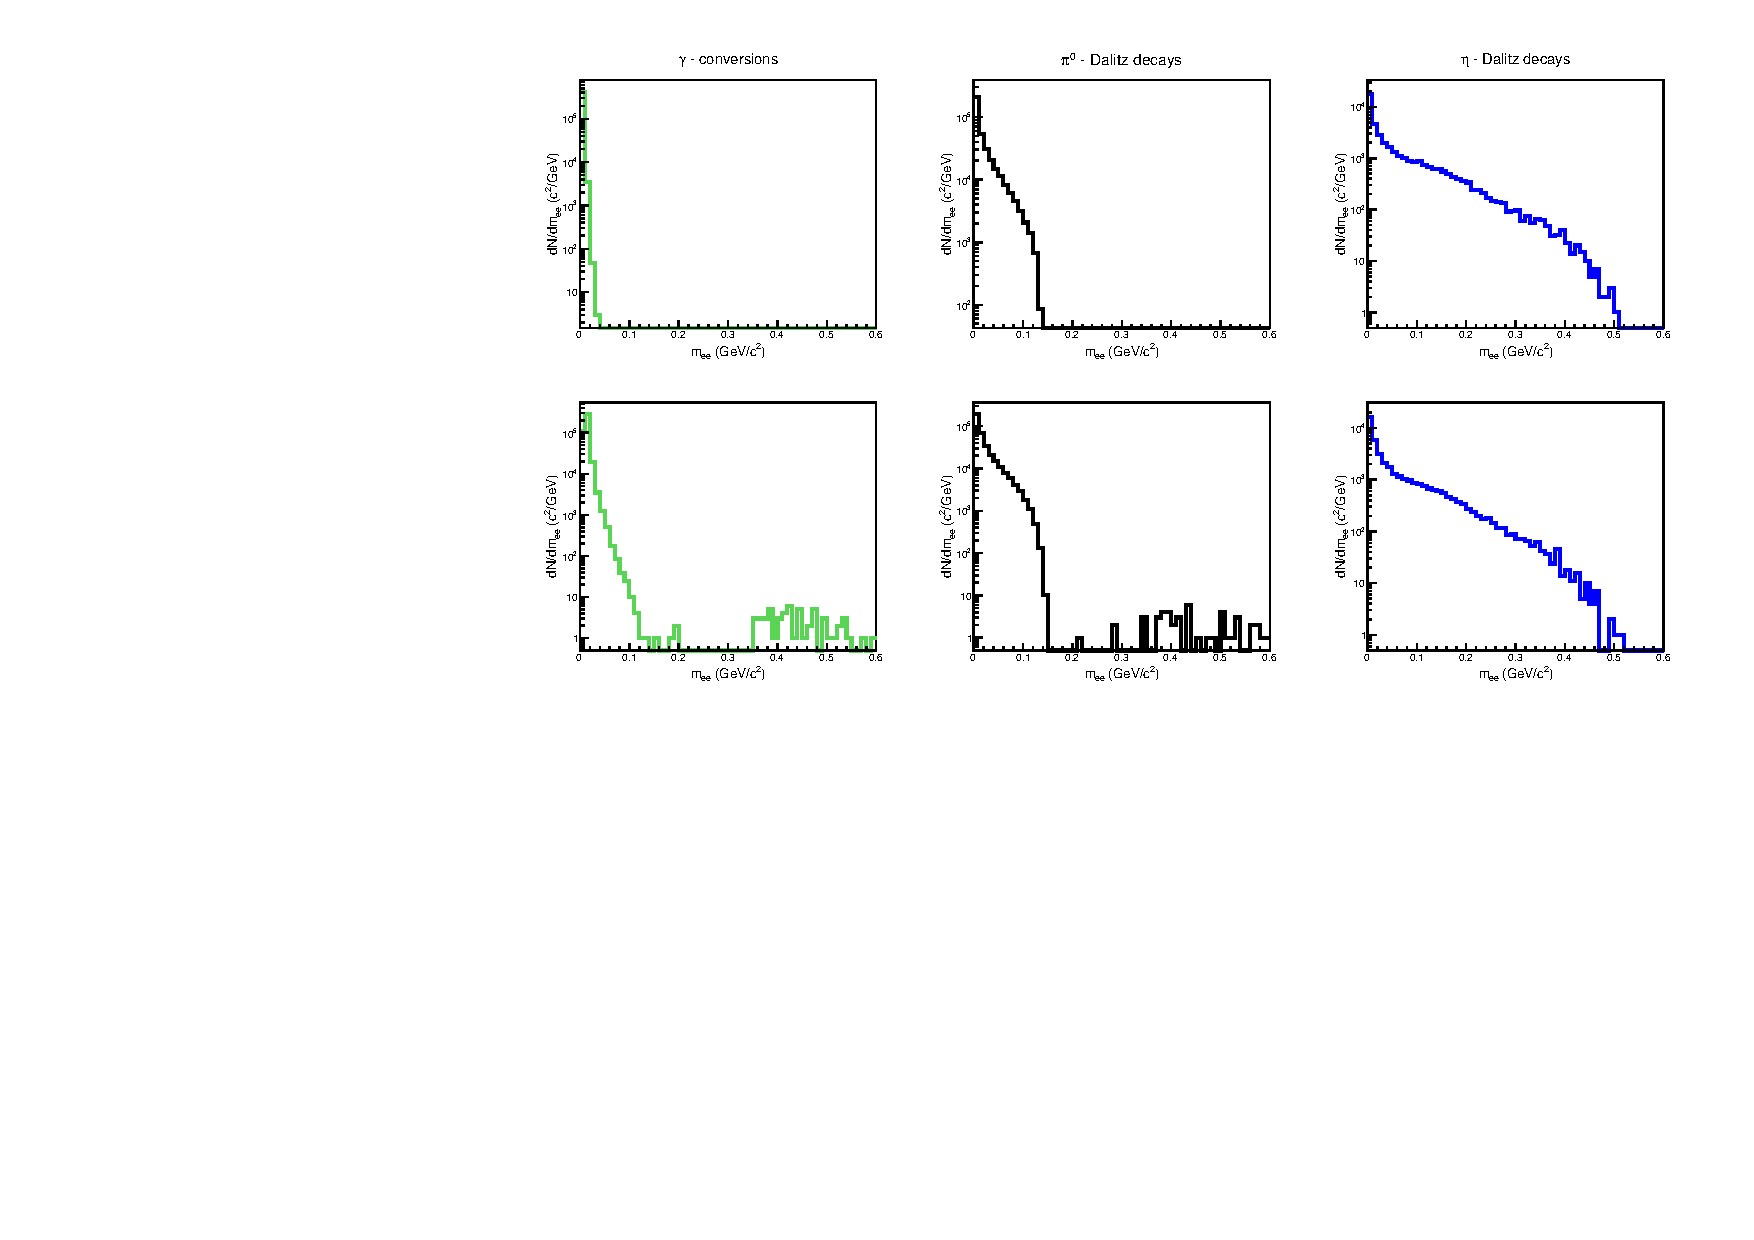
\includegraphics[scale = 0.8]{sources2.pdf}
\caption{The invariant mass distributions of photon conversions (green), $\pi^{0}$ Dalitz decay (black) and $\eta$ Dalitz decay (blue). 
The upper plots are obtained with MC parameters while the lower ones with ESD parameters.}
\label{invariant_mass}
\end{center}
\end{figure*}

Considering only the invariant mass it is then possible to obtain the invariant mass distribution for each source. From these we 
can have the information of the shape of the distribution and of the number of particles detected. In Fig. \ref{invariant_mass} are shown 
the invariant mass distributions of the three sources: in the upper line they have been obtained using the MC truth parameters, while
in the lower one from the ESD reconstructed tracks parameters. 
Thus we can notice how the distributions obtained from the reconstructed tracks of the particles are wider than the others,
due to the finite resolution of the detectors.
The numbers of $\gamma$ conversions, $\pi^{0}$ and $\eta$ Dalitz decays, known from MC truth, are shown in the following table:

\begin{table}[htb]
\center
\caption{Amount of $e^{+}e^{-}$ pairs from the three sources, obtained from the MC information}\label{amount_MC}
\begin{tabular}{|c|c|}
  \hline
  \raisebox{0pt}[12pt ][6pt]{number of $\gamma$} &
  \raisebox{0pt}[12pt][6pt]{418300 $\pm$ 600} \\
  \hline
  \raisebox{0pt}[12pt][6pt]{number of $\pi^{0}$} &
  \raisebox{0pt}[12pt][6pt]{362000 $\pm$ 600} \\
  \hline
  \raisebox{0pt}[12pt][6pt]{number of $\eta$} &
  \raisebox{0pt}[12pt][6pt]{42100 $\pm$ 200} \\
  \hline
  \raisebox{0pt}[12pt][6pt]{$n_{\gamma}/ n_{\pi^{0}}$} &
  \raisebox{0pt}[12pt][6pt]{1.156 $\pm$ 0.003} \\
  \hline
  \raisebox{0pt}[12pt][6pt]{$n_{\gamma}/ n_{\eta}$} &
  \raisebox{0pt}[12pt][6pt]{9.94 $\pm$ 0.05} \\
  \hline
  \raisebox{0pt}[12pt][6pt]{$n_{\gamma}/(n_{\pi^{0}}+n_{\eta})$} &
  \raisebox{0pt}[12pt][6pt]{1.035 $\pm$ 0.002} \\
  \hline
  \end{tabular}
\end{table}

We are especially interested in the ratios, in fact the aim of this study is to find a fit template which can separate the three sources 
from the inclusive $p_{T}$ spectrum and quantify the ratios between them.\\

It is finally possible to put together the three contributions, that should represent the majority of the background (at least for 
$m_{ee} < m_{\eta}$), and fit the result with a parametric function, which summarises the three contributions.

\subsection{Fitting functions}

The parameterization is different for photon conversions and Dalitz decays.\\
For the first source an exponentially modified Gaussian distribution has been chosen, 
\vspace{0.2cm}
\begin{equation}
\frac{dN}{dm_{ee}}=N_{\gamma}\cdot e^{-\frac{(m_{ee}-M_{\gamma})^{2}}{2\sigma^{2}}}+\Theta(m_{ee}-M_{\gamma})
e^{\frac{m_{ee}-M_{\gamma}}{\tau}}
\label{gaussexp}
\end{equation}
\vspace{0.2cm}

where $\Theta$ is the Heaviside function, which is defined equal to zero for $m_{ee} < M_{\gamma}$ and equal to 1 for 
$m_{ee} > M_{\gamma}$.\\

The resulting function is shown in Fig. \ref{photon_conversions}.
This function fits reasonably well because the invariant mass of a photon is not exactly zero, in fact the conversion can only happen
near to a nucleus, which transfers a fraction of his momentum. In addition for the reconstructed tracks it is necessary to take into 
consideration the finite resolution of the detectors.\\

\begin{figure}[htb]
\begin{center}
\advance\leftskip-0.5cm
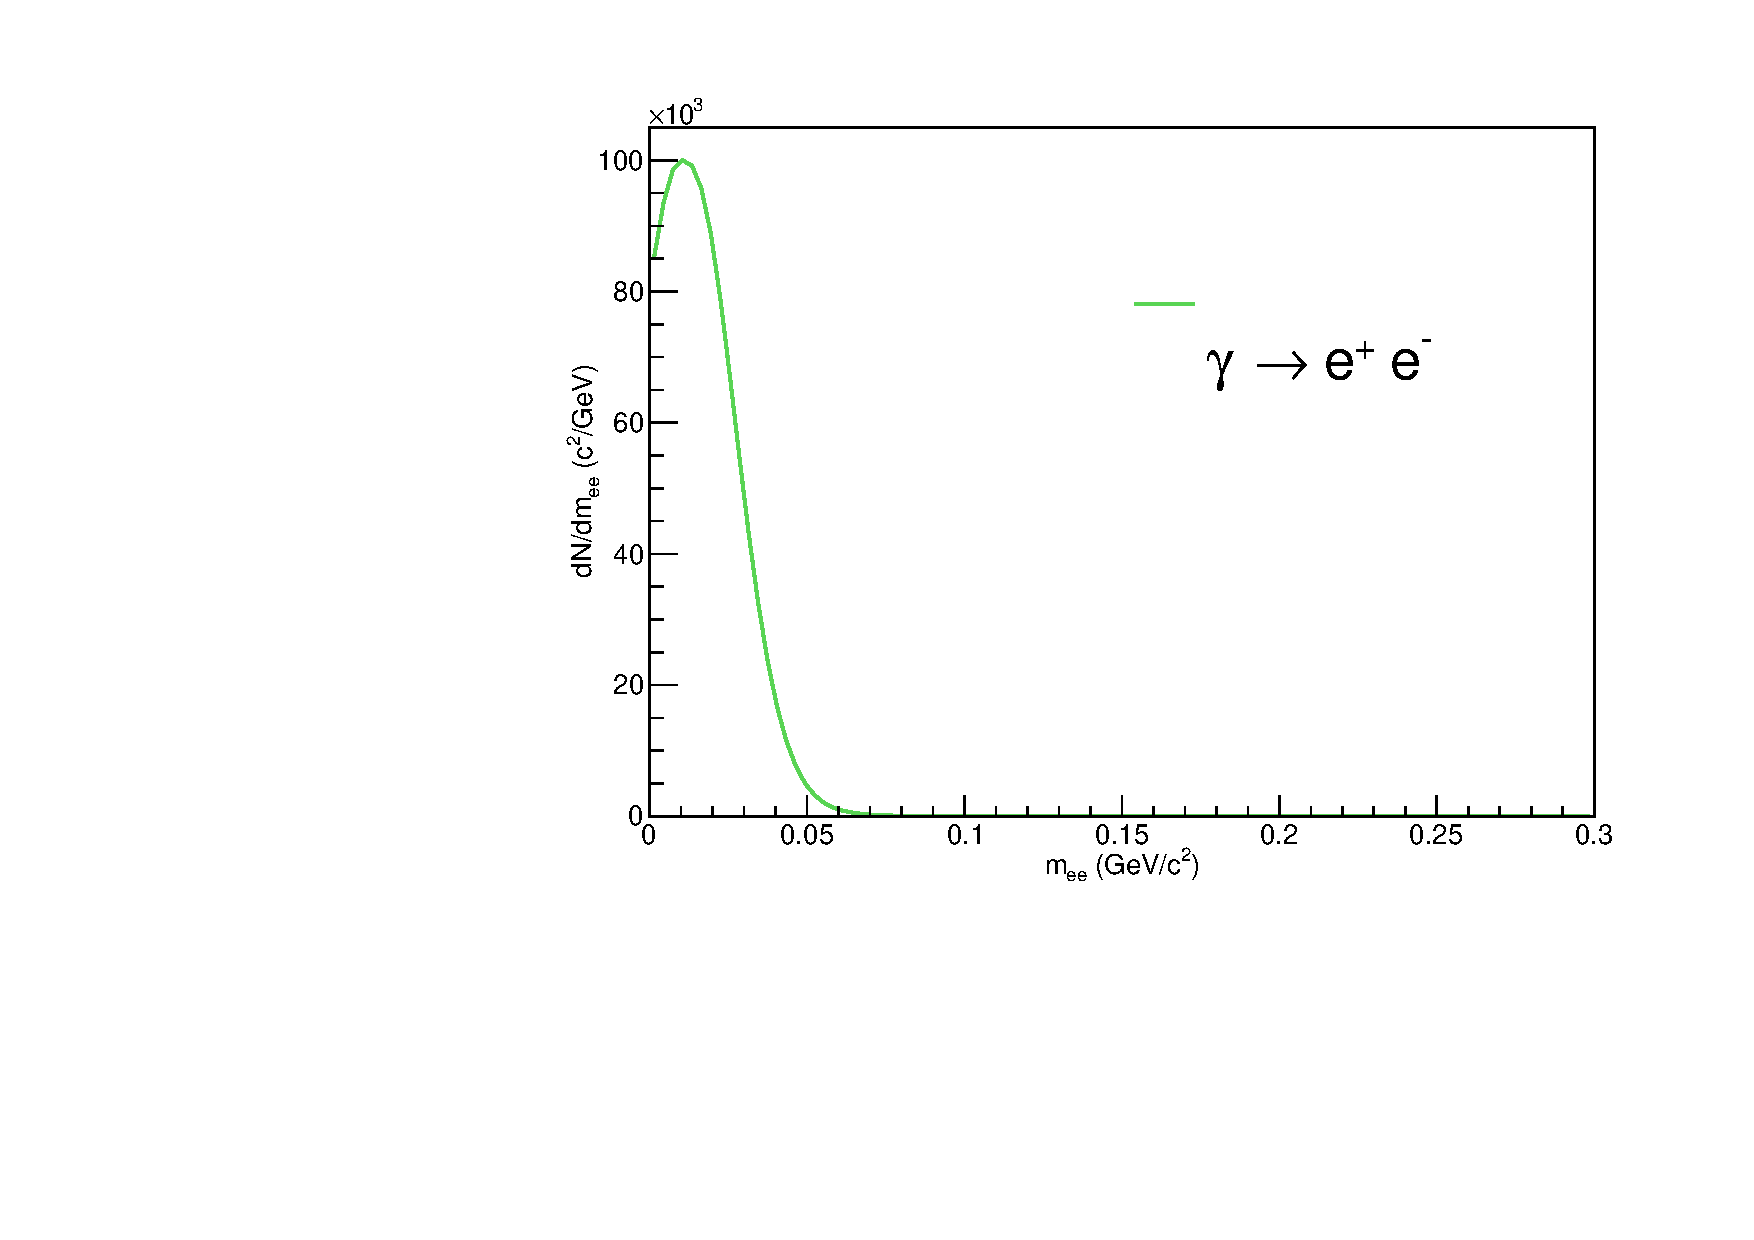
\includegraphics[scale = 0.4]{gamma_temp.pdf}
\caption{The function used to describe the invariant mass distribution for photon conversions.}
\label{photon_conversions}
\end{center}
\end{figure}

For the Dalitz decays, instead, the \\Kroll-Wada distribution, which is the proper distribution to describe these kind
of decays, has been used:

\vspace{0.2cm}
\begin{equation}
\begin{split}
\frac{dN}{dm_{ee}} &=N_{X}\cdot\frac{2}{m_{ee}}B^{3/2}\sqrt{1-\frac{4(m_{e}/M_{X})^{2}}{(m_{ee}/M_{X})^{2}}}\times \\
&\times \Bigg\{1+\frac{2(m_{e}/M_{X})^{2}}{(m_{ee}/M_{X})^{2}}\Bigg\}\cdot F_{X}(m_{ee}^2) 
\label{kroll_wada}
\end{split}
\end{equation}
\vspace{0.2cm}

where $N_{X}$ is a normalisation factor, $m_{e}$ is the mass of an electron or a positron, $M_{X}$ the mass of the mother particle.
The mass of the mother particle determines the width of the distribution. In fact, as we can see in Fig. \ref{kroll-wada}, the 
distribution for the $\eta$ meson is wider then the one for the $\pi^{0}$ because the first one has a mass of about $m_{\eta} \simeq 547.85$ 
MeV, while the second one has $m_{\pi^{0}} \simeq 139.57$ MeV.

In the formula also appears the factor B, which is equal to:
\vspace{0.2cm}
\begin{equation}
B=(1+(m_{ee}/M_{X})^{2})^2-4(m_{ee}/M_{X})^{2}.
\label{kroll_wada}
\end{equation}
\vspace{0.2cm}

Finally the Form Factor $F_{X}$ is different for every Dalitz decay. For the $\pi^{0}$ and the $\eta$ the expressions are respectively:

\vspace{0.2cm}
\begin{equation}
\Bigg\{
\begin{array}{rl}
F_{\pi^{0}}(m_{ee}^2) = \frac{1}{(1-5.5\cdot m_{ee}^2)^{2}}\\
F_{\eta}(m_{ee}^2) = \frac{1}{(1-1.9\cdot m_{ee}^2)^{2}}
\label{formfactors}
\end{array}
\end{equation}

\begin{figure}[htb]
\begin{center}
\advance\leftskip-0.5cm
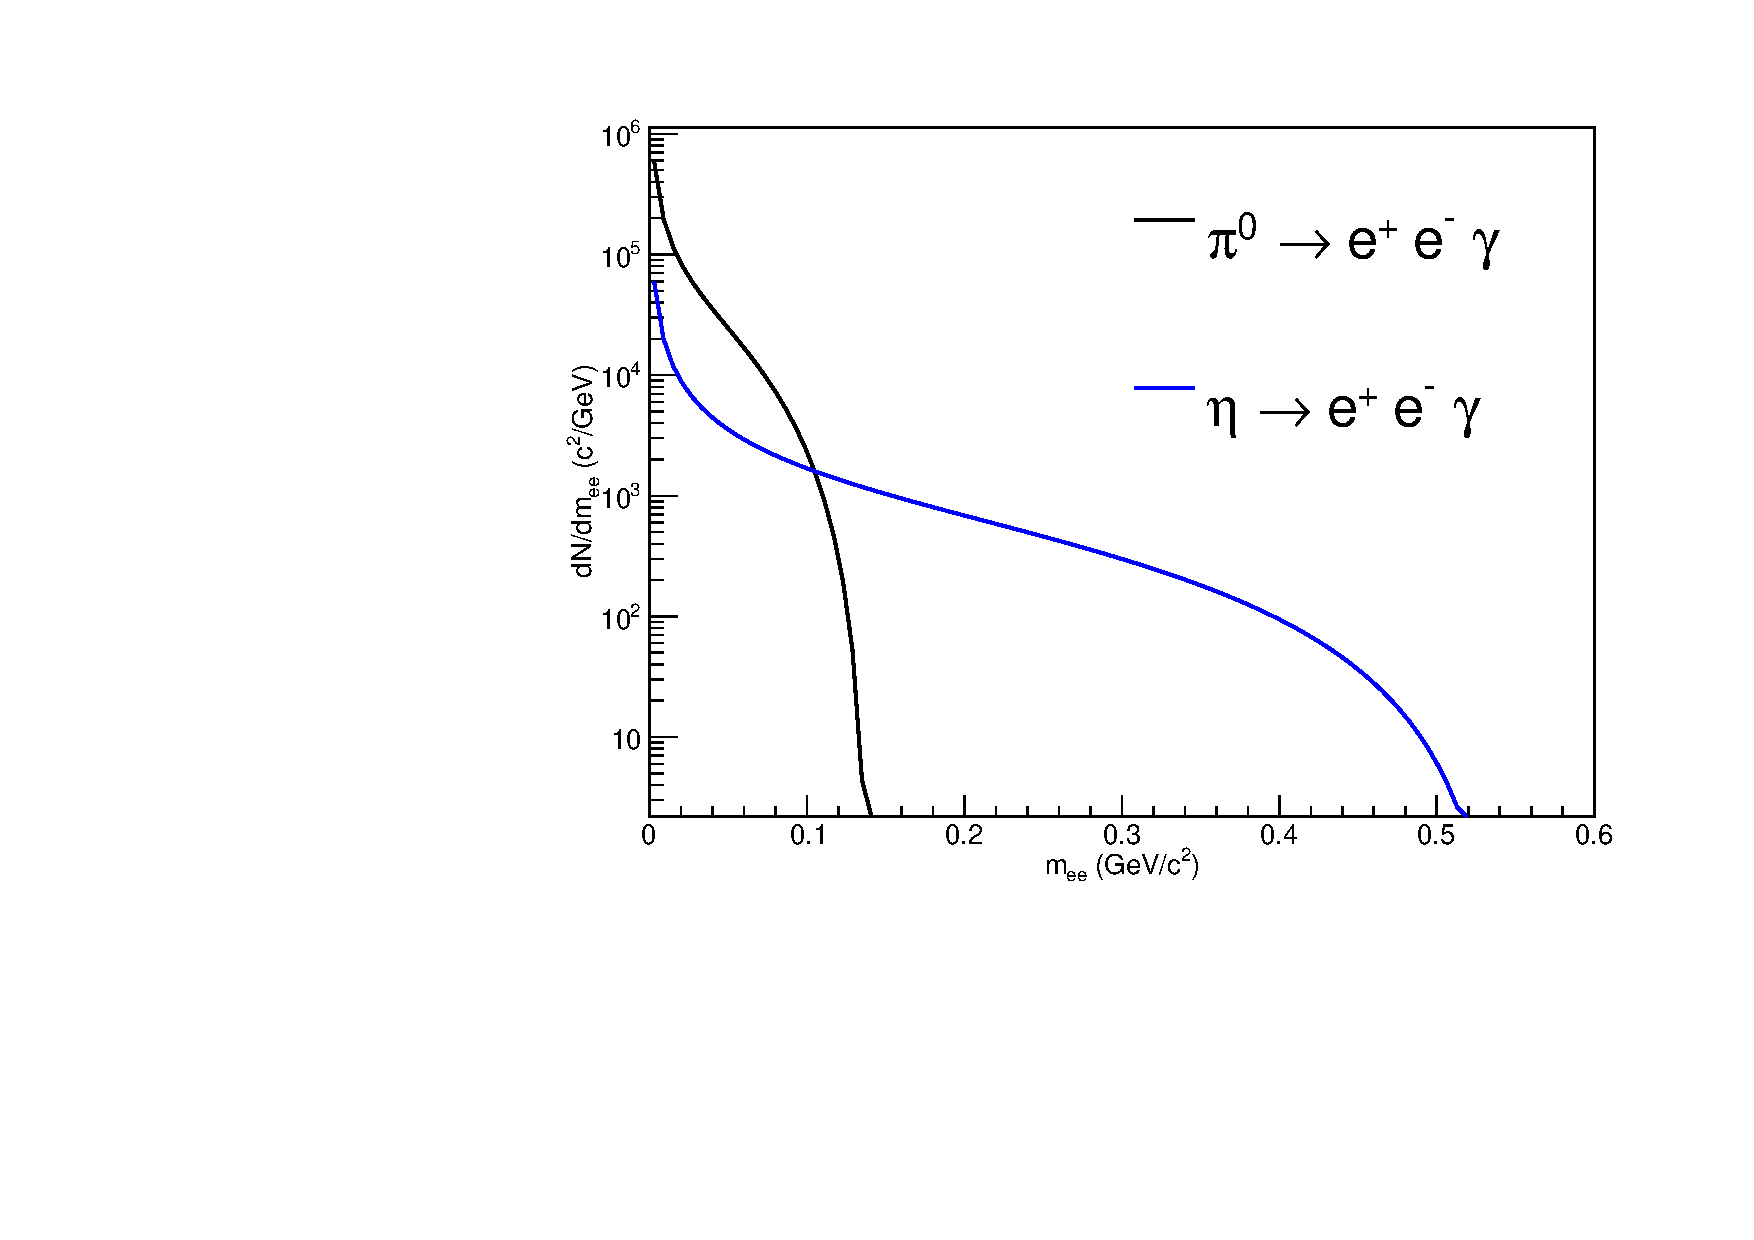
\includegraphics[scale = 0.4]{dalitz_temp.pdf}
\caption{The Kroll-Wada distributions for $\pi^{0}$ Dalitz decays and $\eta$ Dalitz decays.}
\label{kroll-wada}
\end{center}
\end{figure}

\subsection{Fit of the photonic background with MC information}
\label{subsec:fit}
With the purpose of fitting the photonic signal, the three invariant mass distributions of the main sources have been put together and 
fitted with a function, which is the sum of the three contributions described in the previous section. In order to simulate the photonic
signal, measured with the real detector, the distributions obtained from the ESD reconstructed tracks have been considered.\\
The aim of this section is to verify that it is possible to obtain the amount (and then the relative ratios) of the three sources, 
performing a fit and integrating the three separated contributions, in which the parameters have been fixed from the fit done with the 
composed function. In this analysis the parameters which should represent the mass of the mothers have been left free and fixed 
subsequently from the fit. 
These values extrapoleted from the fit are higher then the real masses of the two mesons, in fact the distributions of the Dalitz decays 
cannot be properly described by the Kroll-Wada, due to the fact that some counts for low transverse momentum and low invariant mass are 
lost, because particles with low $p_{T}$ and $m_{ee}$ cannot reach the detectors.\\
This problem affects more the $\pi^{0}$ distribution than the $\eta$ one, because the $\pi^{0}$ meson has a lower mass (the real values 
are $m_{\pi^{0}} \simeq 139.57$ MeV and $m_{\eta} \simeq 547.85$ MeV).

\begin{figure*}[tb]
\center
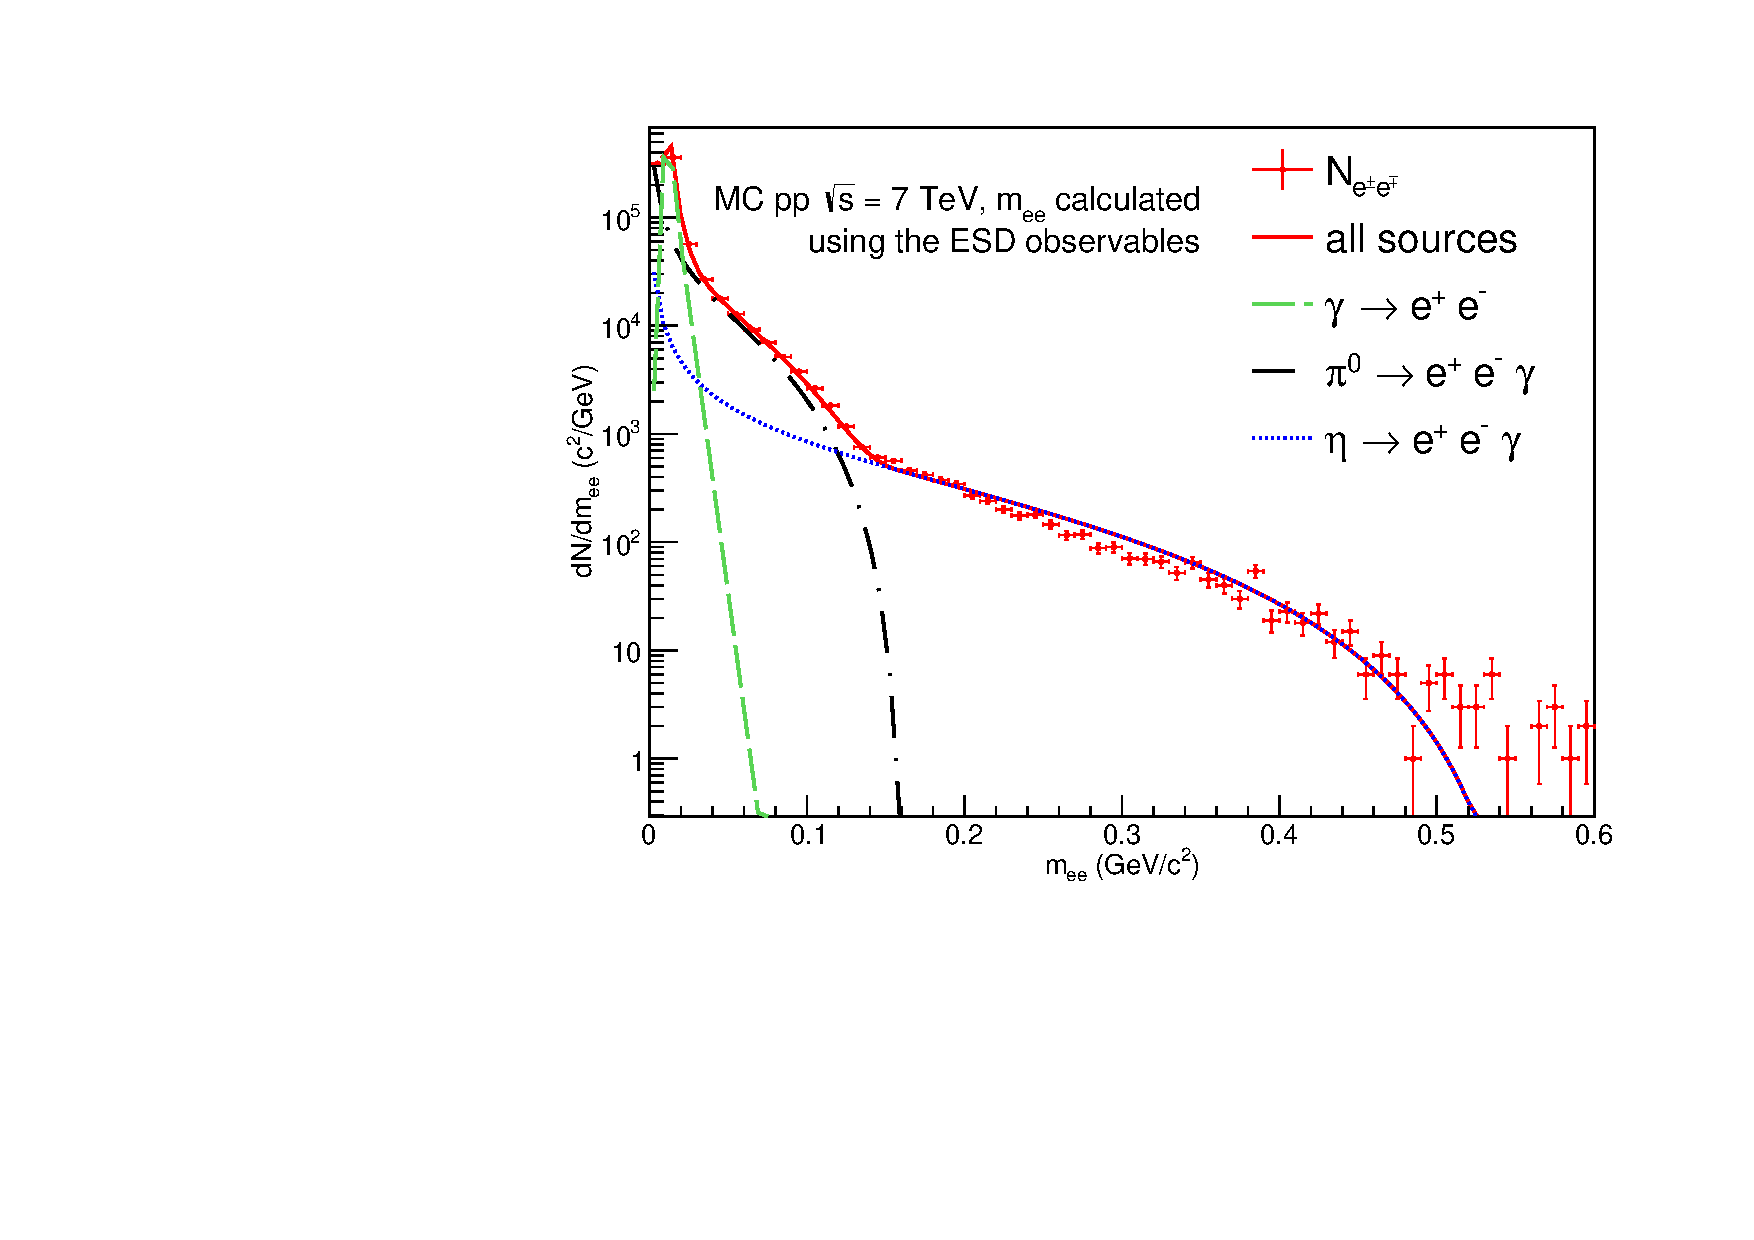
\includegraphics[scale = 0.7]{Inv_mass_ESD.pdf}
\caption{Invariant mass distribution for $\gamma$ conversion, $\pi^{0}$ and $\eta$ Dalitz decays from MC truth with 
observables from ESD reconstructed tracks. The red line represent the composed function wich has been used to perform the fit.
The other functions correspond to the single sources. Once obtained they have been integrated in the invariant mass range of interest, 
in order to obtain the amount of the three distinct contributions.}
\label{ESDdist}
\end{figure*}

The photonic signal obtained in this way and the relative fit are shown in Fig. \ref{ESDdist}.\\

The values of the parameters from the fit and the integrals of the single contributions are summarised in Tab.\ref{fit}.
\begin{table}[htpb]
\center
\caption{Amount of $e^{+}e^{-}$ pairs from the three sources, obtained from the fit of the MC distribution}\label{fit}
\begin{tabular}{|c|c|}
  \hline
  \raisebox{0pt}[10pt][6pt]{$M_{\gamma}$} &
  \raisebox{0pt}[10pt][6pt]{0.01107 $\pm$ 0.00018 $GeV/c^{2}$} \\
  \hline
  \raisebox{0pt}[10pt][6pt]{$M_{\pi^{0}}$} &
  \raisebox{0pt}[10pt][6pt]{0.1611 $\pm$ 0.0003 $GeV/c^{2}$} \\
  \hline
  \raisebox{0pt}[10pt][6pt]{$M_{\eta}$} &
  \raisebox{0pt}[10pt][6pt]{0.558 $\pm$ 0.004 $GeV/c^{2}$} \\
  \hline
  \raisebox{0pt}[10pt][6pt]{Integral of $\gamma$ } &
  \raisebox{0pt}[10pt][6pt]{418300 $\pm$ 1100} \\
  \hline
  \raisebox{0pt}[10pt][6pt]{Integral of $\pi^{0}$ } &
  \raisebox{0pt}[10pt][6pt]{355000 $\pm$ 2000} \\
  \hline
  \raisebox{0pt}[10pt][6pt]{Integral of $\eta$ } &
  \raisebox{0pt}[10pt][6pt]{49200 $\pm$ 600} \\
  \hline
  \raisebox{0pt}[10pt][6pt]{$I_{\gamma}/I_{\pi^{0}}$} &
  \raisebox{0pt}[10pt][6pt]{1.179 $\pm$ 0.007} \\
  \hline
  \raisebox{0pt}[10pt][6pt]{$I_{\gamma}/I_{\eta}$} &
  \raisebox{0pt}[10pt][6pt]{8.50 $\pm$ 0.11} \\
  \hline
  \raisebox{0pt}[10pt][6pt]{$I_{\gamma}/(I_{\pi^{0}}+I_{\eta})$} &
  \raisebox{0pt}[10pt][6pt]{1.035 $\pm$ 0.006} \\
  \hline
  \end{tabular}
\end{table}

If we compare these results with the numbers of particles known from MC truth, which are summarised in Table \ref{amount_MC}, we can 
immediatly notice that the number of photon conversions is well described with this method. For the Dalitz decays there is a little
discrepancy, in particular we obtained less $\pi^{0}$ and more $\eta$ mesons. Anyway the sum of the two contributions is consistent 
with the MC information, which probably means that some $\pi^{0}$ mesons have been misidentified as $\eta$ mesons in the low invariant 
mass region.

\section{Photonic background without MC information}
\subsection{Like-sign and unlike-sign distributions}

\begin{figure*}[tb]
\center
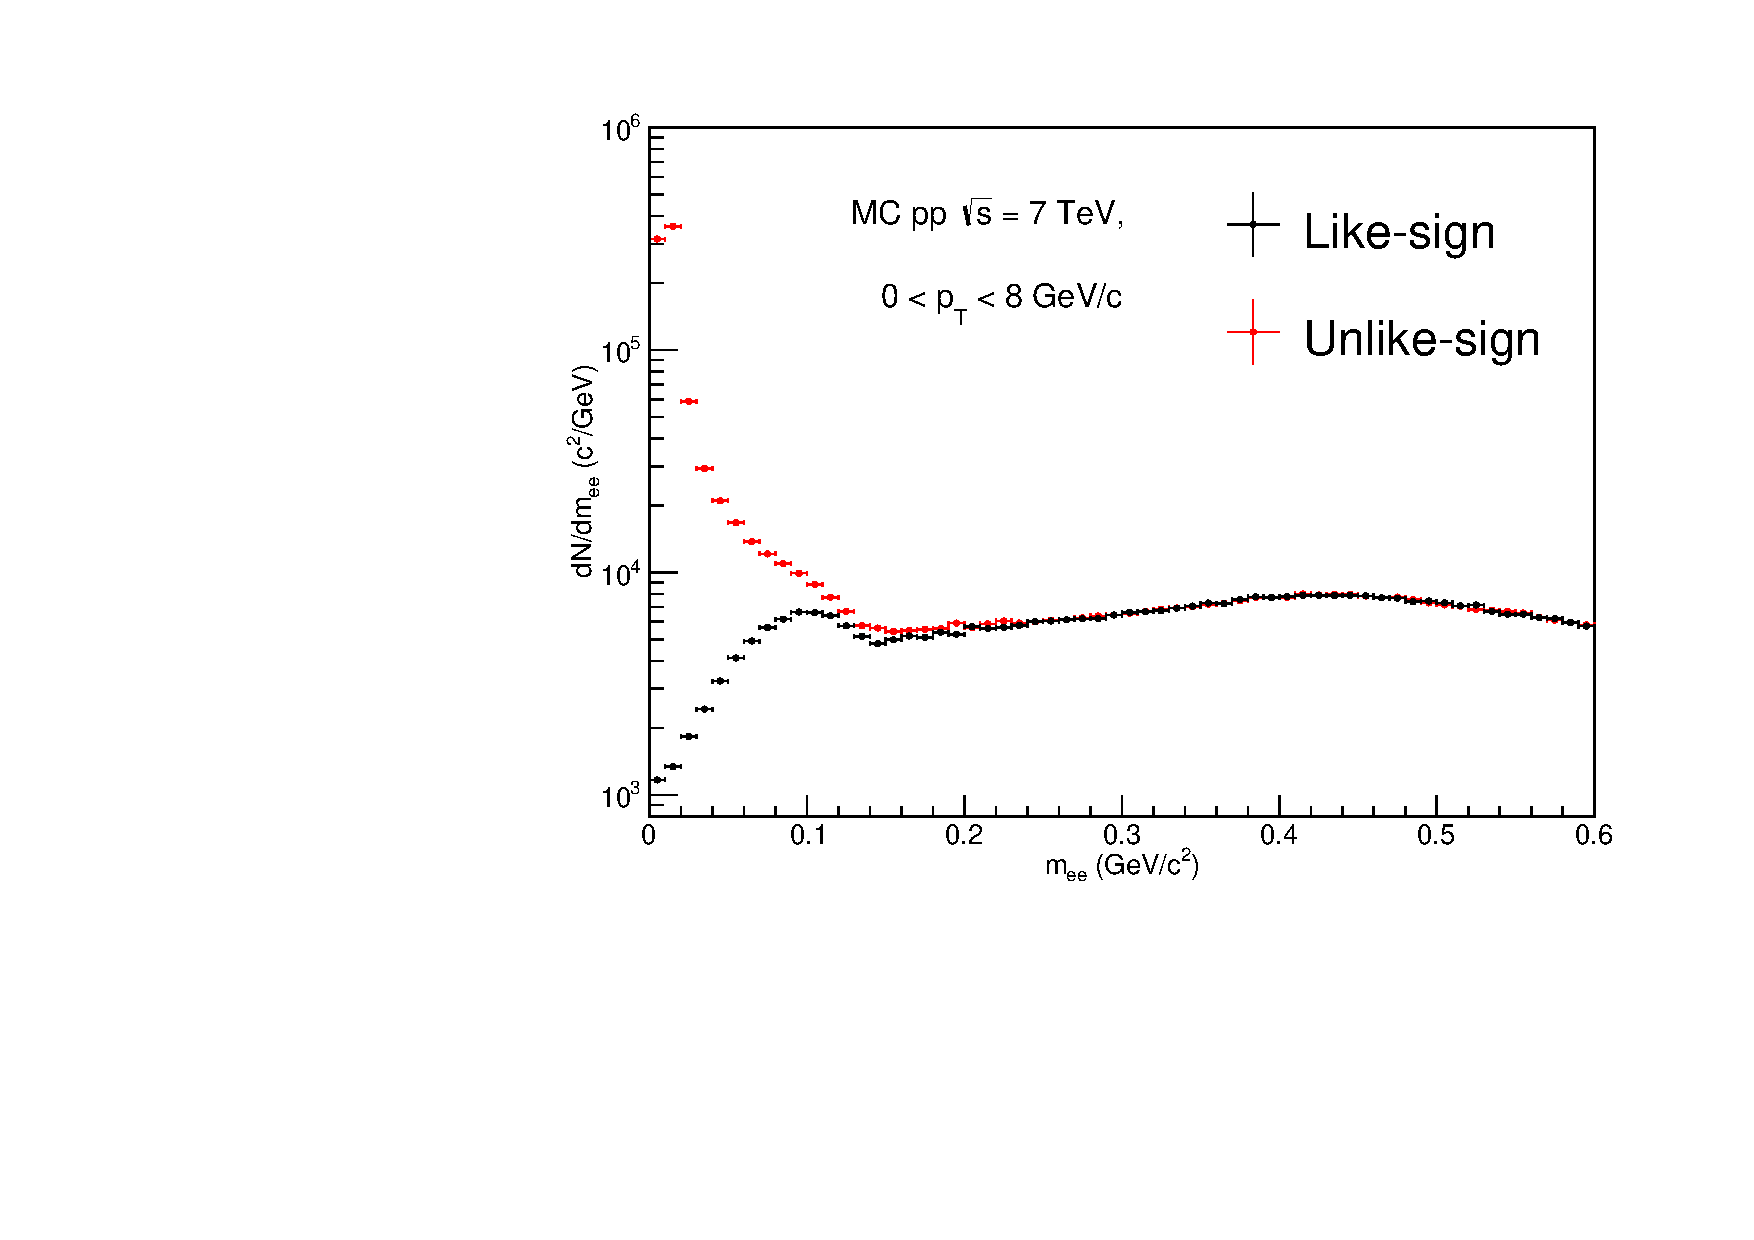
\includegraphics[scale = 0.7]{like-unlike_norm.pdf}
\caption{The invariant mass distribution of like-sign ($e^{\pm}e^{\pm}$) and unlike-sign ($e^{\pm}e^{\mp}$) combination.}
\label{LSUS}
\end{figure*}

In order to approach a realistic analysis strategy to be performed with real data, the MC truth information is ignored in this section.\\
Therefore every "inclusive" $e^{\pm}$ is combined to an "associated" $e^{\mp}$ and for each pair the invariant mass $m_{ee}$ is 
calculated to create the unlike-sign distribution, that contains both the photonic signal, and the combinatorial background. \\
Then every "inclusive" $e^{\pm}$ is paired to an "associated" $e^{\pm}$ for the like-sign invariant mass distribution. 
This one represents only the combinatorial background, that will be then subtracted from the unlike-sign distribution to obtain only 
the signal which we are interested in.\\

\begin{figure}[htb]
\center
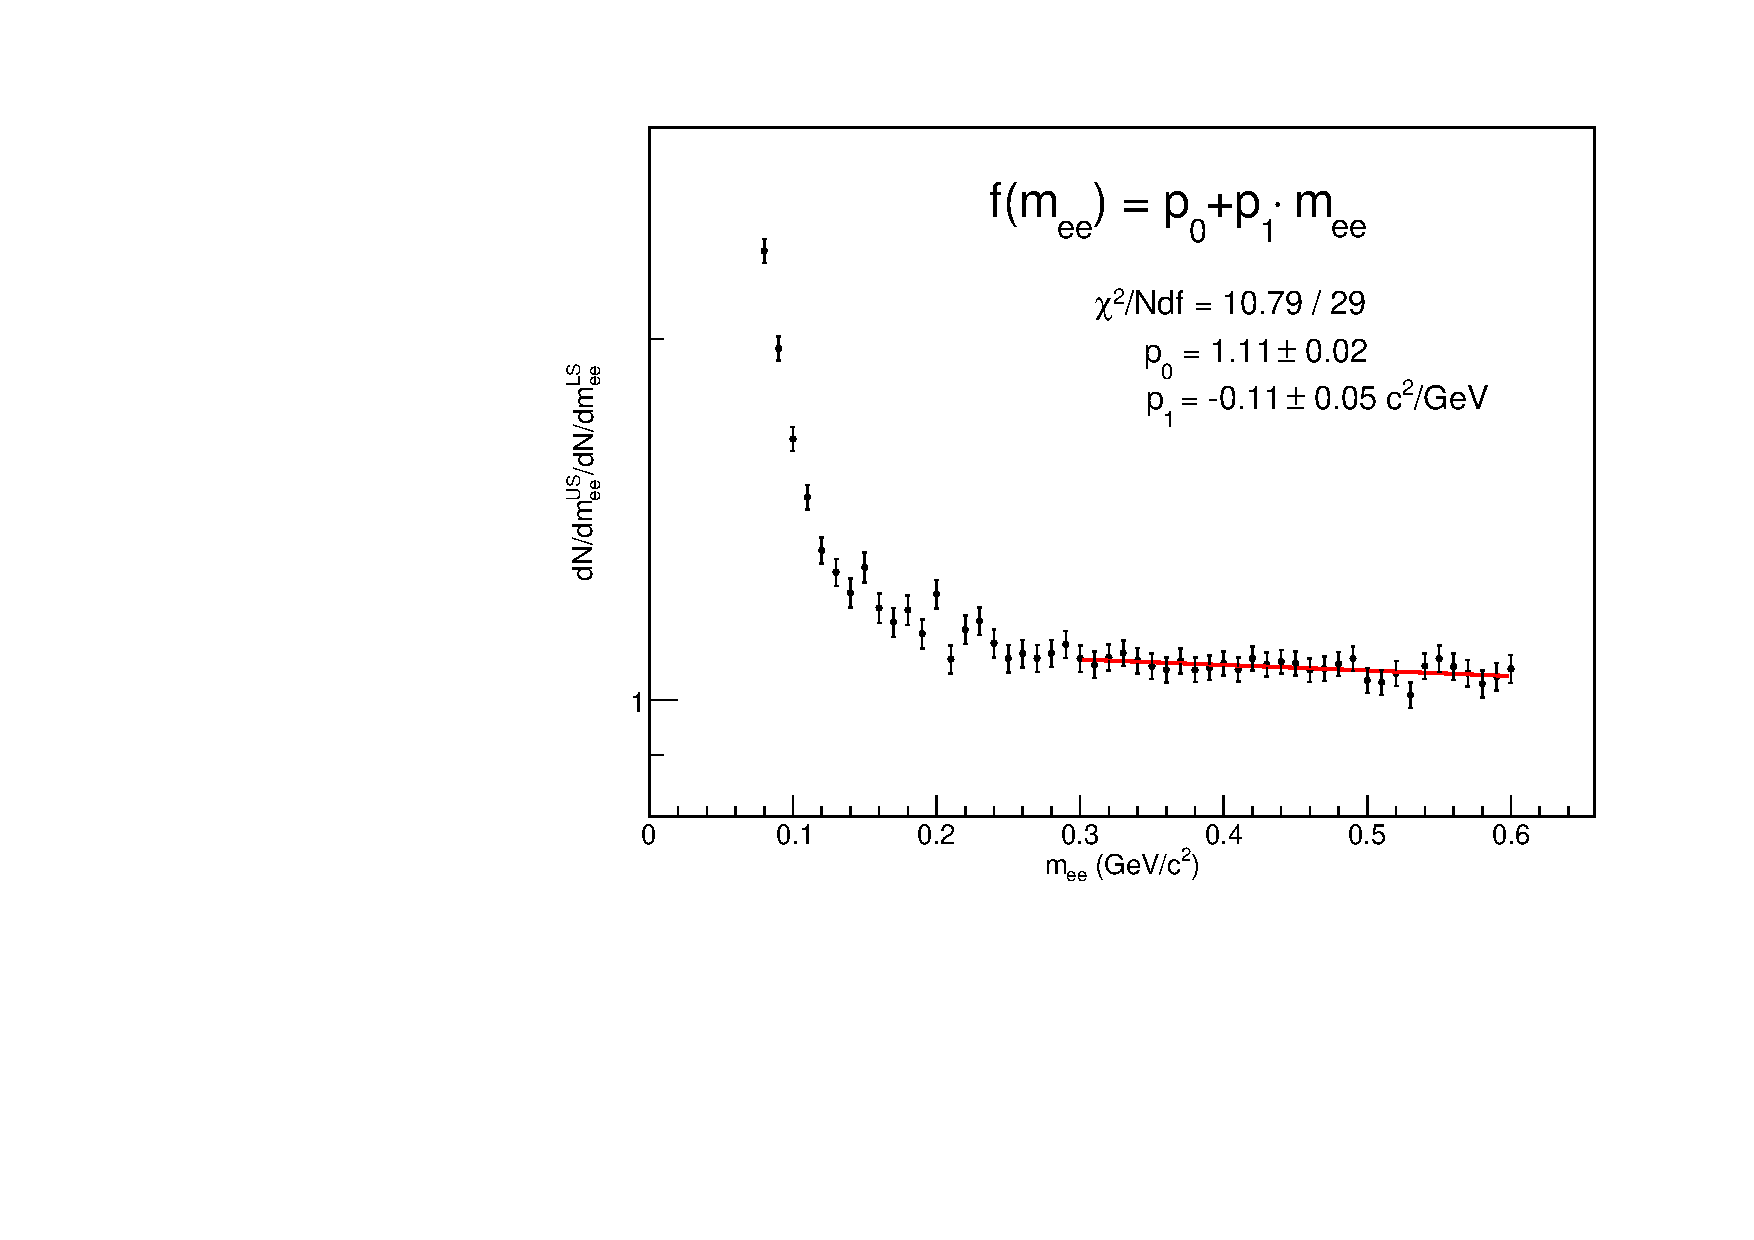
\includegraphics[scale = 0.4]{USLS_ratio.pdf}
\caption{The invariant mass distribution of like-sign ($e^{\pm}e^{\pm}$) and unlike-sign ($e^{\pm}e^{\mp}$) combination.}
\label{LSUS}
\end{figure}

In Fig. \ref{LSUS} the two distributions are shown: the red points belong to the 
unlike-sign distribution, the black ones to the like-sign distribution.\\
For the like-sign distribution a normalisation was necessary, in fact not all the combinatorial background was subtracted.\\

Therefore for every bin the ratio between the unlike-sign and the like-sign distribution has been calculated, and then linearly fitted 
starting from $m_{ee} >$ 0.3 $GeV/c^{2}$.
Every bin of the like-sign distribution has been then multiplied for the value of the line in the centre of the bin, to obtain the 
normalised distribution.\\

\subsection{Fit of the photonic background without MC information}

\begin{figure*}[tb]
\center
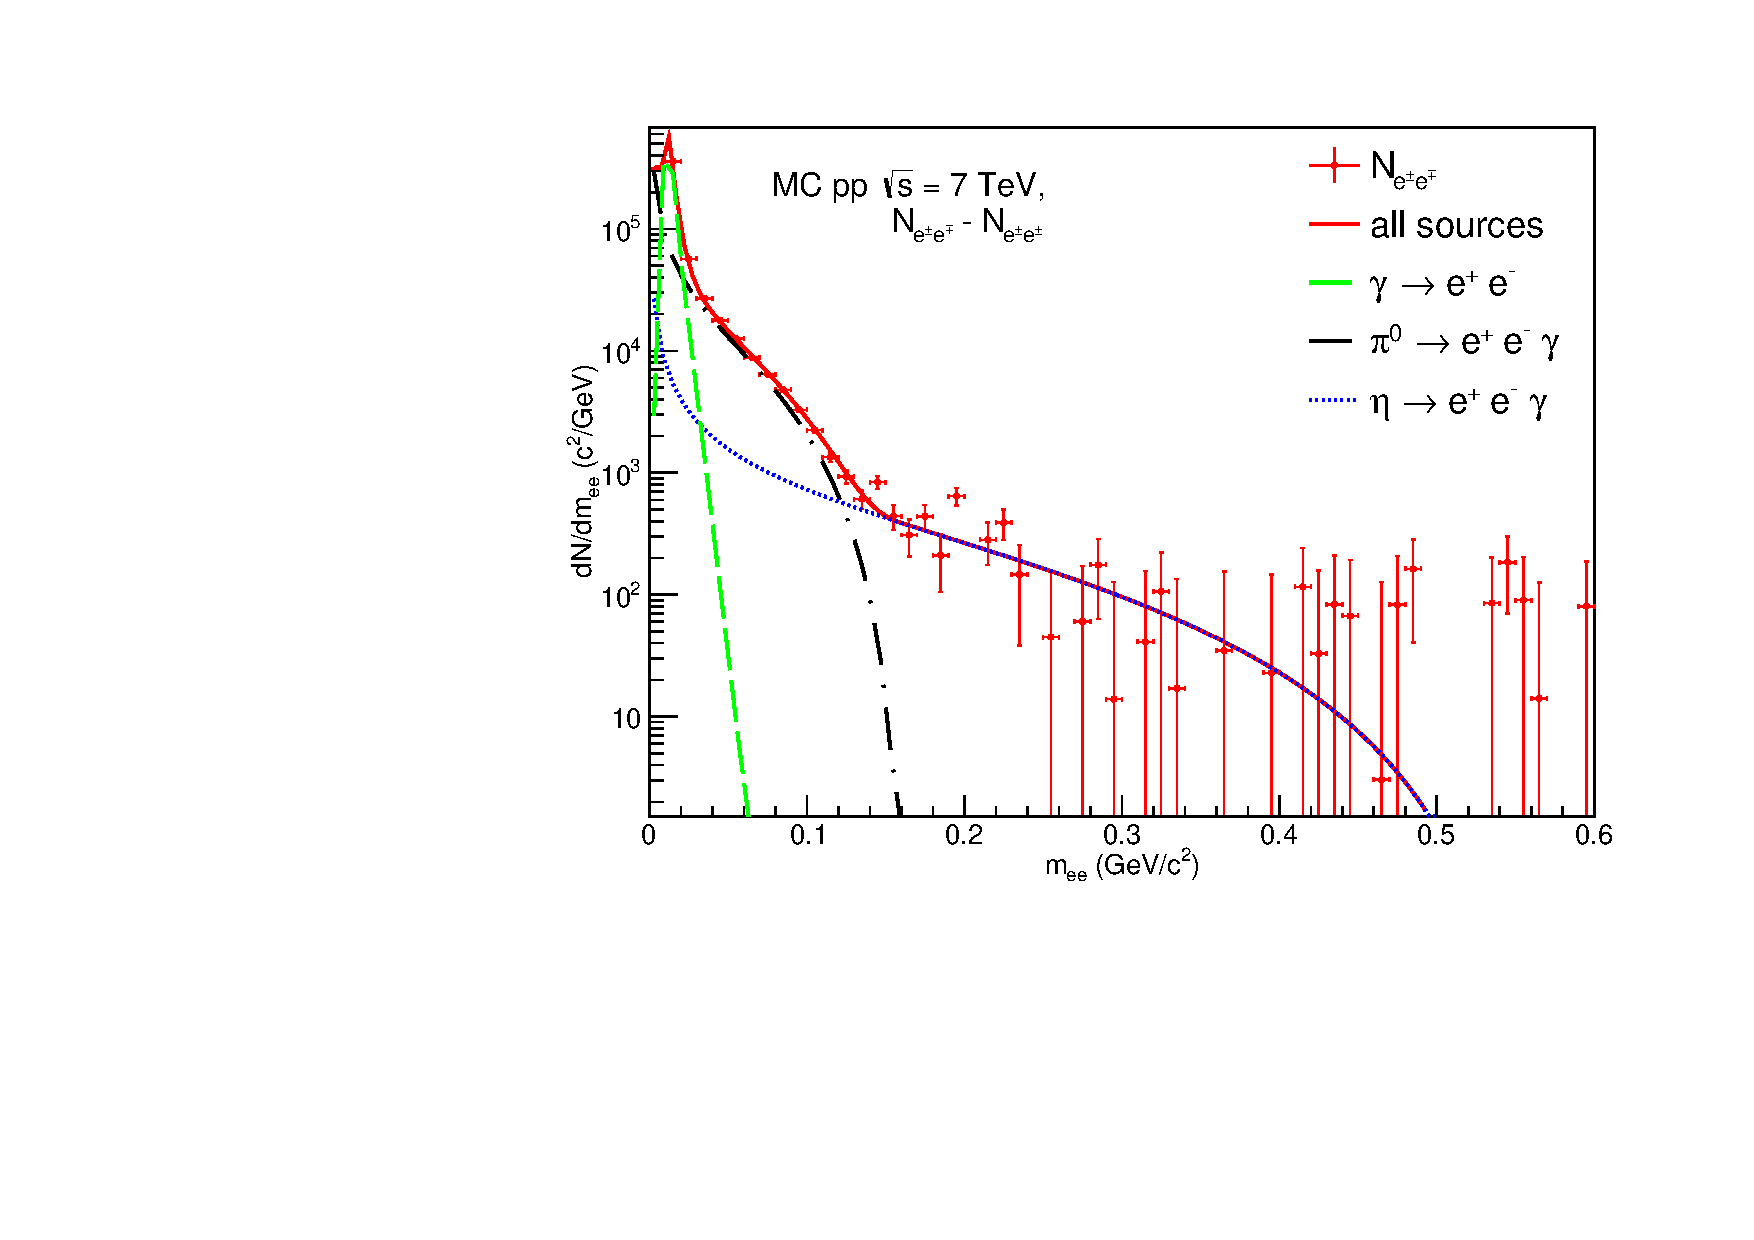
\includegraphics[scale=0.7]{esd_comb.pdf}
\caption{The photonic background fitted with the template obtained from the MC truth.}
\label{photonic}
\end{figure*}

Once subtracted the like-sign distribution from the unlike-sign, the resulting photonic background has been fitted with the templates 
extrapolated from the MC truth in section \ref{subsec:fit}, as represented in Fig. \ref{photonic}.
The values of the parameters that should represent the masses have been fixed from the ones obtained from the previous fit (Table 
\ref{fit}).\\
The purpose of this method is therefore to obtain the same amount of $\gamma$, \space $\pi^{0}$ and $\eta$, as known from the MC truth.
The integral of the three contributions and the relative ratios are shown in the following table:

\begin{table}[htpb]
\center
\caption{Amount of $e^{+}e^{-}$ pairs from the three sources, obtained from the fit of the photonic background}\label{fit2}
\begin{tabular}{|c|c|}
  \hline
  \raisebox{0pt}[10pt][6pt]{Integral of $\gamma$ } &
  \raisebox{0pt}[10pt][6pt]{423000 $\pm$ 6000} \\
  \hline
  \raisebox{0pt}[10pt][6pt]{Integral of $\pi^{0}$ } &
  \raisebox{0pt}[10pt][6pt]{354000 $\pm$ 4000} \\
  \hline
  \raisebox{0pt}[10pt][6pt]{Integral of $\eta$ } &
  \raisebox{0pt}[10pt][6pt]{42000 $\pm$ 3000} \\
  \hline
  \raisebox{0pt}[10pt][6pt]{$I_{\gamma}/I_{\pi^{0}}$} &
  \raisebox{0pt}[10pt][6pt]{1.19 $\pm$ 0.02} \\
  \hline
  \raisebox{0pt}[10pt][6pt]{$I_{\gamma}/I_{\eta}$} &
  \raisebox{0pt}[10pt][6pt]{10.0 $\pm$ 0.8} \\
  \hline
  \raisebox{0pt}[10pt][6pt]{$I_{\gamma}/(I_{\pi^{0}}+I_{\eta})$} &
  \raisebox{0pt}[10pt][6pt]{1.07 $\pm$ 0.02} \\
  \hline
  \end{tabular}
\end{table}

As we can see the values obtained from the fit are comparable to the real ones known from the MC truth, within the statistical error.

\section{Conclusions and Outlook}
The goal was to determine the ratio between the contribution from photon conversions and from $\pi^{0}$ and $\eta$ Dalitz decays 
to the photonic background to the electrons from heavy-flavor hadron decays.\\ 
It has been reached, although more precise results could be obtained fixing some details (for example the problem of higher masses).
The ratio between $\gamma$ and $\eta$ seems to be the best one to be considered, but it is only due to the large statistical error.
In fact the relative error for the number of $\eta$ is of 7.1\%, while for $\pi^{0}$ is 1.1\% and for $\gamma$ 1.4\%.\\ 
Therefore the ratio between photon conversions and all the contributes from Dalitz decays should be used.
Moreover we can notice that some counts from $\pi^{0}$ could be misidentified and contribute to the $\eta$ integral, as it was 
already discussed in section \ref{subsec:fit}). The total number of Dalitz decays has not changed anyway.\\

The next step would be look into real proton-proton data, to see if the same ratio is found.
Finally, the same study can be applied to Pb-Pb data, to verify that there is an excess of $\gamma$, which are supposed to be 
thermal photons originated by the fireball, which is only created in heavy ions ultra-relativistic collision.  
More information about this phenomenon can be found in the article \cite{Masciocchi:2011fu}.

\section*{Acknowledgements}
I would like to thank all the ALICE group at GSI, for their support, their kindness and their availability at any time.
Working with them has been always pleasant and enjoyable.\\
I am especially grateful to Ralf Averbeck, my supervisor, Silvia Masciocchi, Jochen Th\"{a}der, Maria Nicassio, Jan Wagner, Ana Marin,
Dariusz Miskowiec and Lukas Kreis; they were always present and they always helped me when needed.
I want also to thank J\"{o}rn Knoll, Marina Varentsova and all the other organizers of the Summer Student Program for the chance 
that they gave me to participate in it. 

\begin{thebibliography}{99}

\bibitem{Averbeck:2013oga}
  R.~Averbeck,
  %``Heavy-flavour production in heavy-ion collisions and implications for the properties of hot QCD matter,''
  Prog.\ Part.\ Nucl.\ Phys.\  {\bf 70} (2013) 159.
  %%CITATION = PPNPD,70,159;%%
  %3 citations counted in INSPIRE as of 02 Sep 2014

\bibitem{Abelev:2012xe}
  B.~Abelev {\it et al.}  [ALICE Collaboration],
  %``Measurement of electrons from semileptonic heavy-flavour hadron decays in pp collisions at \sqrt{s} = 7 TeV,''
  Phys.\ Rev.\ D {\bf 86} (2012) 112007
  [arXiv:1205.5423 [hep-ex]].
  %%CITATION = ARXIV:1205.5423;%%
  %48 citations counted in INSPIRE as of 02 Sep 2014

\bibitem{Andronic:2014zha}
  A.~Andronic,
  %``An overview of the experimental study of quark-gluon matter in high-energy nucleus-nucleus collisions,''
  arXiv:1407.5003 [nucl-ex].
  %%CITATION = ARXIV:1407.5003;%%
  
\bibitem{Schukraft:2011na}
  J.~Schukraft [ALICE Collaboration],
  %``Heavy Ion physics with the ALICE experiment at the CERN LHC,''
  Phil.\ Trans.\ Roy.\ Soc.\ Lond.\ A {\bf 370} (2012) 917
  [arXiv:1109.4291 [hep-ex]].
  %%CITATION = ARXIV:1109.4291;%%
  %3 citations counted in INSPIRE as of 02 Sep 2014

\bibitem{Landsberg:1986fd}
  L.~G.~Landsberg,
  %``Electromagnetic Decays of Light Mesons,''
  Phys.\ Rept.\  {\bf 128} (1985) 301.
  %%CITATION = PRPLC,128,301;%%
  %243 citations counted in INSPIRE as of 02 Sep 2014
  
\bibitem{Masciocchi:2011fu}
  S.~Masciocchi [ALICE Collaboration],
  %``Investigation of charm and beauty production via semileptonic decays of heavy-flavour hadrons in pp at 7 TeV and Pb--Pb at 2.76 TeV with ALICE,''
  J.\ Phys.\ G {\bf 38} (2011) 124069
  [arXiv:1109.6436 [nucl-ex]].
  %%CITATION = ARXIV:1109.6436;%%
  %15 citations counted in INSPIRE as of 04 Sep 2014
  
\bibitem{ex:schm} C.A. Schmidt, Photonic background measurement for electrons from semileptonic heavy-flavour decays with ALICE at the 
LHC, {\it Master thesis} (2013) 

\end{thebibliography}

\end{document}